\documentclass[10pt, conference, letterpaper]{IEEEtran}
\mathchardef\Gamma="0100 \mathchardef\Delta="0101
\mathchardef\Theta="0102 \mathchardef\Lambda="0103
\mathchardef\Xi="0104 \mathchardef\Pi="0105
\mathchardef\Sigma="0106 \mathchardef\Upsilon="0107
\mathchardef\Phi="0108 \mathchardef\Psi="0109
\mathchardef\Omega="010A

\newcommand{\ovspace}[1]{\vspace{#1}}

\newcommand{\outline}[1]{}%{\textbf{#1}}

\newcommand{\dl}{\mbox{$\, [ \hspace*{-1.5pt} [\,$}}
\newcommand{\dr}{\mbox{$\, ] \hspace*{-1.5pt} ]\:$}}
\newcommand{\da}{\mbox{$\, A \hspace*{-6.75pt} A \,$}}
%\newcommand{\drightarrow}{\mbox{$\rightarrow \hspace*{-8pt} \rightarrow$}}

\newcommand{\BA}{\mbox{${\bm{a}}$}}
%\newcommand{\BB}{\mbox{${\bm{c}}$}}
\newcommand{\BC}{\mbox{${\bm{c}}$}}
\newcommand{\BD}{\mbox{${\bm{d}}$}}
\newcommand{\BE}{\mbox{${\bm{e}}$}}
\newcommand{\BO}{\mbox{${\bm{o}}$}}
\newcommand{\BP}{\mbox{${\bm{p}}$}}
\newcommand{\BQ}{\mbox{${\bm{q}}$}}
\newcommand{\BR}{\mbox{${\bm{r}}$}}
\newcommand{\BV}{\mbox{${\bm{v}}$}}
\newcommand{\BL}{\mbox{${\bm{l}}$}}
\newcommand{\BI}{\mbox{${\bm{i}}$}}
\newcommand{\BH}{\mbox{${\bm{h}}$}}
\newcommand{\BS}{\mbox{${\bm{s}}$}}
\newcommand{\BB}{\mbox{${\bm{k}}$}}

\newcommand{\wrapbox}[1]{\framebox{\begin{tabular}{c}#1\end{tabular}}}
\newcommand{\CodeIn}[1]{{\small\texttt{#1}}}
\newcommand{\Section}[1]{Section~\ref{sec:#1}}
\newcommand{\SFigure}[2]{Figure~\ref{fig:#1}(#2)}

\usepackage{cite}
\usepackage{xspace}
\usepackage{url}
\usepackage{graphicx}
\usepackage{latexsym}
\usepackage{amssymb}
\usepackage{amsfonts}
%\usepackage{times}
\usepackage{psfrag}
%\usepackage{subfigure}
\usepackage{wrapfig}
\usepackage{comment}
%packages for algorithms
%\usepackage{algorithm}
%\usepackage{algorithmic}
\usepackage{alltt}
\usepackage{color}

\newtheorem{defn}{Definition}[section]
\newtheorem{exmp}{Example}[section]
\newtheorem{thrm}{Theorem}[section]
\newtheorem{prop}{Proposition}[section]
\newtheorem{lemm}{Lemma}[section]
\newtheorem{obsv}{Observation}[section]
\newtheorem{corr}{Corollary}[section]

%\addtolength{\textheight}{.23in} \addtolength{\textwidth}{.15in}
%\addtolength{\topmargin}{-.23in}
%\addtolength{\oddsidemargin}{.1in}
%\addtolength{\evensidemargin}{.1in}

\newtheorem{thm}{Theorem}
\newtheorem{dfn}{Definition}
\newtheorem{lem}{Lemma}
\newtheorem{cor}{Corollary}
\newcommand{\ie}{\emph{i.e.}\xspace}
\newcommand{\eg}{\emph{e.g.}\xspace}
\newcommand{\etc}{\emph{etc.}\xspace}
\newcommand{\etal}{\frenchspacing{}\emph{et al{.}}\xspace}
%\newcommand{\etal}[1]{{\sl et al.{#1}}}

%\newcommand{\thm}[1]{Theorem~\ref{thm:#1}}
%\newcommand{\lem}[1]{Lemma~\ref{lemma:#1}}
%\newcommand{cor}[1]{Corollary~\ref{cor:#1}}
\newcommand{\fac}[1]{Fact~\ref{fact:#1}}
\newcommand{\Table}[1]{Table~\ref{tab:#1}}
\newcommand{\Figure}[1]{Figure~\ref{fig:#1}}

%\theoremstyle{plain}
\newtheorem{property}{Property}[section]
\newtheorem{lemma}{Lemma}[section]
\newtheorem{corollary}{Corollary}[section]
\newtheorem{theorem}{Theorem}[section]

%\theoremstyle{definition}
\newtheorem{notation}{Notation}
\newtheorem{Definition}{Definition}[section]

%\theoremstyle{remark}
\newtheorem{fact}{Fact}[section]
\newtheorem{observation}{Observation}[section]
\newtheorem{insight}{Insight}[section]

%%\algorithmstyle{definition}
%\algsetup{indent=1em}
%\renewcommand{\algorithmicrequire}{\textbf{Input:  }}
%\renewcommand{\algorithmicensure}{\textbf{Output:}}
\newcommand{\factorial}{\ensuremath{\mbox{\sc Factorial}}}

\newcommand{\Comment}[1]{}

\renewcommand\floatpagefraction{0.999}
\renewcommand\topfraction{0.999}
\renewcommand\bottomfraction{0.999}
\renewcommand\textfraction{0.001}
\setcounter{totalnumber}{5}

\usepackage{amsthm}
\usepackage{mathtools}
\usepackage{balance}
\usepackage[margin=0.15in]{caption}
%\usepackage[cmex10]{amsmath}
%\usepackage[lined, boxed, comments numbered, ruled]{algorithm2e}

%% INFOCOM 2013 addition:
\makeatletter
\def\ps@headings{%
\def\@oddhead{\mbox{}\scriptsize\rightmark \hfil \thepage}%
\def\@evenhead{\scriptsize\thepage \hfil \leftmark\mbox{}}%
\def\@oddfoot{}%
\def\@evenfoot{}}
\makeatother
\pagestyle{headings}
%% END INFOCOM 2013 addition

\newcommand{\figwidth}{0.35\textwidth}
\newcommand{\proc}{Proc. }
\newcommand{\Proc}{Proc. }
\newcommand{\conf}{Conf. }
\newcommand{\Conf}{Conf. }
\newcommand{\inte}{Int. }
\newcommand{\Inte}{Int. }
\newcommand{\Symp}{Symp. }

\newcommand{\presec}{\vspace{0.0in}}
\newcommand{\postsec}{\vspace{0.0in}}
\newcommand{\presub}{\vspace{0.0in}}
\newcommand{\postsub}{\vspace{0.0in}}

\newcommand{\tabincell}[2]{\begin{tabular}{@{}#1@{}}#2\end{tabular}}

\newcommand{\prefig}{\vspace{-0.06in}}
\newcommand{\postfig}{\vspace{-0.06in}}
\newcommand{\adjustfigs}{\vspace{0.1in}}

\newcommand{\precaption}{\vspace{-0.06in}}
\newcommand{\postcaption}{\vspace{-0.06in}}
\newcommand{\preequation}{\vspace{-0in}}
\newcommand{\postequation}{\vspace{-0in}}
\newcommand{\prefigcaption}{\vspace{-0in}}
\newcommand{\subfigs}{\hspace{-0in}}
\newcommand{\subfigsvert}{\vspace{-0in}}
\newcommand{\pretheorem}{\vspace{-0in}}
\newcommand{\posttheorem}{\vspace{-0in}}

\newcommand{\figwidthdraw}{0.4\textwidth}
\newcommand{\figwidtheva}{0.3\textwidth}




\graphicspath{{./FigDrawing/},{./FigEvaluation/},{./EvaluateFigures/}}

	\clubpenalty=10000
	\widowpenalty = 10000

%%%%%%%%%%%%%%%%%%%%%%%%%%%%%%%%%%%%%%%%%%%%%%%%%%%%%%%%%%%%%%%%%%%%%%%%%%%%%%%%%%%
% Journal version idea : Alex Liu
% 1. Extend the FP calculation to other types of Bloom filters such as counting BF.
%
%
%%%%%%%%%%%%%%%%%%%%%%%%%%%%%%%%%%%%%%%%%%%%%%%%%%%%%%%%%%%%%%%%%%%%%%%%%%%%%%%%%%%

\title{On the Controversy of Bloom Filter False Positives - An Information Theoretical Approach to\\Optimizing Bloom Filter Parameters}

%\author{Paper \#517, \: 9 pages}
%\Comment{
%\author{\IEEEauthorblockN{Michael Shell\IEEEauthorrefmark{1},
%Homer Simpson\IEEEauthorrefmark{2},
%James Kirk\IEEEauthorrefmark{3},
%Montgomery Scott\IEEEauthorrefmark{3} and
%Eldon Tyrell\IEEEauthorrefmark{4}}
%\IEEEauthorblockA{\IEEEauthorrefmark{1}School of Electrical and Computer Engineering\\
%Georgia Institute of Technology,
%Atlanta, Georgia 30332--0250\\ Email: see http://www.michaelshell.org/contact.html}
%\IEEEauthorblockA{\IEEEauthorrefmark{2}Twentieth Century Fox, Springfield, USA\\
%Email: homer@thesimpsons.com}
%\IEEEauthorblockA{\IEEEauthorrefmark{3}Starfleet Academy, San Francisco, California 96678-2391\\
%Telephone: (800) 555--1212, Fax: (888) 555--1212}
%\IEEEauthorblockA{\IEEEauthorrefmark{4}Tyrell Inc., 123 Replicant Street, Los Angeles, California 90210--4321}}
%}

\begin{document}

\maketitle

\begin{abstract}
%
Although Bloom Filters (BF) have been widely used in many networking applications and beyond, the fundamental issue of how to calculate the false positive probability remains elusive.
%
Properly calculating the false positive probability of BF is critical because it is used to calculate the optimal number of hash functions $k$.
%
Since Bloom gave the false positive formula in 1970, in 2008, Bose \textit{et al.} pointed out that Bloom's formula for calculating the false positive probability is flawed and gave a new false positive formula; and in 2010, Christensen \etal further pointed out that Bose's formula is also flawed and gave another new false positive formula.
%
Although Christensen's formula is perfectly accurate, it is time-consuming to calculate the false positive probability, and it is impossible to calculate the derivation of the optimal value of $k$.
%
While the conventional wisdom is to derive the optimal value of $k$ from a false positive formula, in this paper, we propose the first approach to calculating the optimal $k$ without any false positive formula.
%
Our approach is based on the following observation: for a BF with $m$ bits and $n$ elements, if and only if its entropy is the largest, its false positive probability is the smallest, according to information entropy theory.
%
Furthermore, we propose a new and more accurate upper bound for the false positive probability.
%
When the size of a Bloom filter becomes infinitely large, our upper bound turns equal to the lower bound, which becomes Bloom's formula.
%
This deepens our understanding of Bloom's formula: it is perfectly accurate when $m$ is infinitely large, and it is practically accurate when $m$ is sufficiently large.
%
Besides, we derive the bounds of correct rate of counting Bloom filters (one widely used variant of BFs for estimating item frequencies) by applying our proposed formulas about BFs to them. 
% 
We release our source code of Bloom Filters in \cite{opensource} without any identity information.
\end{abstract}

%\vspace{0.15in}
%\begin{IEEEkeywords}
%Bloom Filter, False Positive Probability, Information Entropy
%\end{IEEEkeywords} 
\vspace{0.08in}
\presec \section{Introduction} \postsec
\vspace{0.06in}
\subsection{Motivation} \postsub
\vspace{0.06in}
%
A Bloom Filter (BF) is a compact data structure used for quickly checking whether an element belongs to a set or not \cite{BF1970}.
%
Given a set $S$ of $n$ elements, we create a bit array $A$ of length $m$ as follows.
%
First, we initialize each bit of $A$ to 0, then for each element $x \in \mathcal{S}$, we use $k$ hash functions to compute $k$ hash values: $h_1(x), h_2(x),..., h_{k}(x)$ where each hash value is in the range $[1, m]$.
%
Second, for each $1 \leqslant i \leqslant k$, we let $A[h_i(x)]=1$.
%
The resulting bit array $A$ is called the BF for set $S$.
%
To query whether $y \in S$, we first use the same $k$ hash functions to compute $k$ hash values: $h_1(y), h_2(y),..., h_{k}(y)$.
%
Second, we check whether the corresponding $k$ bits in $A$ are all $1s$ (\ie, whether $A[h_1(y)] \wedge A[h_2(y)] \wedge \cdots, A[h_{k}(y)]=1$ holds); if yes, then $y \in S$ may probably hold and we can further check whether $y \in S$; if no, then $y \in S$ definitely does not hold.
%
The cases that the BF shows that $y \in S$ may hold but actually $y \notin S$ are called false positives (FP).
%
The FP probability $f$ can be calculated from $n$, $k$, and $m$.
%
Thus, given a set of $n$ elements and the required FP probability $f$, we can calculate the relationship between $k$ and $m$.
%
Based on the calculated relationship between $k$ and $m$, we can properly trade off between space and speed: smaller $m$ means smaller space, and smaller $k$ means the smaller number of hash function calculations.
%
In typical BF applications, as $m$ is determined by the memory budget for the BF, with known values of $n$ and $f$, we calculate the optimal value for the only unknown parameter $k$.

%%
As set membership query is a fundamental operation in many networking applications, and BFs have the advantages of small memory consumption, fast query speed, and no false negatives, BFs have been widely used in a wide variety of networking applications, such as web caching \cite{webcaching, compressedBFpatent}, IP lookup \cite{sig03PBF, BF_TC, songsig05, HASH-100G}, packet classification \cite{Info04ACPC, Info08memoryPC}, regular expression matching \cite{HPI03deep, HardwareREM}, multicast \cite{BloomCast, Sig02Multicast}, content distribution networks \cite{CDNwww, Sig02informed}, routing \cite{sourceroutingBF, wolfBF}, P2P networks \cite{IAWP2P, P2Psearching}, overlay networks \cite{OverlayMBF, JSAC04Overlay}, name based networks \cite{ BFWY, BFwirelessNDN}, queue management \cite{Info01SFB, Sig06bBF}, Internet measurement \cite{Sig02new, JSAC06measument}, IP traceback \cite{Sig01IPTrace, ICC04scalable}, sensor networks \cite{IPSN07minisec, JSAC05SN}, data center networks \cite{yuConext09, BFDanLi, Info11DCN}, cloud computing \cite{CloudCom11ATree, Cloudcomputingplatform}, cellular networks \cite{PerCom05MANET, WE07securehoc}, and more \cite{shbf, omass}.
%
Most applications with set membership query can potentially be optimized using BFs.

%%
Although BFs have been widely used in many applications, the fundamental issue of how to calculate FP probability remains elusive.
%
Properly calculating the FP probability of BF is critical because it is used to calculate the optimal value of the important parameter $k$, the number of hash functions.
%
In \cite{BF1970}, Bloom gave a formula for calculating the FP probability with known parameters $n$, $k$, and $m$.
%
Based on Bloom's formula, we can also easily compute the optimal value of the parameter $k$ when $m$ and $n$ are known.
%
This formula has been believed to be correct until 2008 when Prosenjit Bose \textit{et al.} pointed out that Bloom's formula is flawed and gave a new FP formula \cite{bose2008false}.
%
Interestingly, two years later, Ken Christensen \textit{et al.} pointed out that Bose's formula is also flawed and gave a new FP formula \cite{ken2010false}.
%
So far, it is believed that Christensen's formula is perfectly accurate.
%
However, Both Bose's and Christensen's FP formulas are too complicated to calculate the optimal value of $k$ from given values of $n$ and $m$.

\presub
\subsection{Main Contributions}\postsub
%%
While the conventional wisdom is to derive the optimal value of BF parameter $k$ from the FP probability, in this paper, we propose the first approach to calculating the optimal $k$ without any FP formula.
%
We first observe that for a BF with $m$ bits and $n$ elements, if and only if its entropy is the largest, its false positive probability is the smallest, according to information entropy theory.
%
Based on this observation, our approach is to derive a formula for calculating the optimal $k$ by letting the entropy equal to 1.
%
We also propose another method to calculate FP probability by deriving the left and right limit expressions of FP probability.
%
We prove that when $m$ goes to infinity, the left and right limits are the same, which is essentially the FP probability.
%
Interestingly, our derived FP formula is the same as Bloom's formula in \cite{BF1970}.
%
This deepens our understanding of Bloom's formula: it is perfectly accurate when $m$ is infinitely large, and it is practically accurate when $m$ is sufficiently large.

%%
In summary, we make three key contributions in this paper.
%
First, we propose an information theoretical approach to calculating the optimal value of BF parameter $k$ without calculating FP probability.
%
Second, we propose a new upper bound which is much more accurate than state-of-the-art.
%
When $m$ is infinitely large, our upper bound becomes the same as the lower bound.
%
This result formally proves that Bloom's formula is practically accurate when $m$ is sufficiently large.
%
Third, we conducted experiments to validate our findings.
%
In particular, we show that the error of Bloom's formula is negligibly small when $m$ is large.
%
Furthermore, we release our source code of Bloom Filters in \cite{opensource} without any identity information.

%
The rest of this paper proceeds as follows.
%
In Section \ref{sec:priorarts}, we introduce the controversy on FP probability.
%
In Section \ref{sec:optimalk}, we show the derivation of the optimal number of hash functions using the information entropy theory.
%
In Section \ref{sec:limitf}, we present a new upper bound of the false positive probability of Bloom Filters.
%
In Section \ref{sec:cbfcr}, we derive the bounds of correct rate of counting Bloom filters through our proposed formulas about Bloom Filters. 
%
In Section \ref{sec:evaluation}, we conduct experiments to evaluate the error of Bloom Filters.
%
%In Section \ref{sec:related}, we discuss related work.
%
We conclude the paper in Section \ref{sec:conclusion}.

\presec \section{Prior Art on BF False Positives} \postsec \label{sec:priorarts}
%
In this section, we review the prior art on calculating the false positive probability of Bloom filters.
%
Table \ref{table:symbols} summarizes the notations used in this paper.

\begin{table} [htbp]
\vspace{0in}
\caption{Notations and abbreviation used in this paper}
\centering
\label{table:symbols}
\begin{tabular}{| c | l |}
\hline Symbol & Description \\
\hline $\mathcal{S}$ & Set of elements\\
\hline $m$  & BF size\\
\hline $n$  & Number of elements in $\mathcal{S}$\\
\hline $k$  & Number of hash functions \\
\hline $k^*$  & Optimal number of hash functions \\
\hline $f$  & False positive probability \\
\hline $f_{bloom}$ & False positive probability calculated by Bloom \\
\hline $f_{bose}$ & False positive probability calculated by Bose \\
\hline $f_{christ}$ & False positive probability calculated by Christensen \\
\hline $f_{true}$        & True false positive probability of BF\\
\hline FP        & false positive\\
\hline BF        & Bloom filter\\
\hline
\end{tabular}
\end{table}

\presub \subsection{Bloom's False Positive Formula} \postsub
%
In 1970, Bloom calculated the false positive probability of a Bloom filter as follows \cite{BF1970}.
%
Given a set $\mathcal{S}$ of elements, let $n$ be the number of elements in $\mathcal{S}$, $k$ be the number of hash functions, and $m$ be the number of bits in the Bloom filter $A$ constructed from set $\mathcal{S}$.
%
In querying an element $x$, the false positive happens when the Bloom filter reports that $x \in \mathcal{S}$ (\ie, $A[h_i(x)]=1$ holds for each $1 \leqslant i \leqslant k$), but actually $x \notin \mathcal{S}$.
%
Consider an arbitrary bit $A[b]$ in $A$.
%
For any element in $\mathcal{S}$ and any hash function $h_i$ ($1 \leqslant i \leqslant k$), the probability that this element is not hashed to bit $A[b]$ by $h_i$ is $1-1/m$.
%
As $\mathcal{S}$ has $n$ elements and each element is hashed $k$ times, the probability of $A[b]=0$ is $p'$:
%
\begin{equation}
p'=\left(1-\dfrac{1}{m}\right)^{kn}
\label{p'form}
\end{equation}
%
Thus, the probability of $A[b]=1$ is $1-(1-1/m)^{kn}$.
%
For any element $x \notin \mathcal{S}$, the probability that the false positive happens for $x$, \ie, the probability of $A[h_1(y)] \wedge A[h_2(y)] \wedge \cdots, A[h_{k}(y)]=1$, is calculated as follows:
%
\begin{equation}
\label{fBloom}
f_{bloom} = \left(1 - \left(1 - \frac{1}{m}\right)^{kn}\right)^k
\end{equation}
%
This formula can be approximated by $(1-e^{\frac{-nk}{m}})^k$, based on which we can trade off between space indicated by $m$ and time indicated by $k$.

\presub
\subsection{Bose's Derivation} \postsub
%
In 2008, Bose \etal pointed out that the last step in Bloom's derivation is flawed because for any element $x \notin \mathcal{S}$, which is hashed into $k$ bits $A[h_1(x)], A[h_2(x)], \cdots, A[h_k(x)]$, the $k$ events $A[h_1(x)]=1, A[h_2(x)]=1, \cdots, A[h_k(x)]=1$ are not actually independent \cite{bose2008false}.
%
Although for each bit $A[h_i(x)]$ ($1 \leqslant i \leqslant k$), after inserting $n$ elements into array $A$, the probability of $A[h_i(x)]=1$ is $1-(1-1/m)^{kn}$, for the probability of $A[h_1(y)] \wedge A[h_2(y)] \wedge \cdots, A[h_{k}(y)]=1$ to be $(1-(1-1/m)^{kn})^k$, the $k$ events $A[h_1(x)]=1, A[h_2(x)]=1, \cdots, A[h_k(x)]=1$ need to be independent.
%
We now analyze the reason that the $k$ events $A[h_1(x)]=1, A[h_2(x)]=1, \cdots, A[h_k(x)]=1$ are not independent.
%
Let us first consider the probability of $A[h_1(x)]=1$, which is $1-(1-1/m)^{kn}$.
%
Second, we consider the probability of $A[h_2(x)]=1$ based on the condition that $A[h_1(x)]=1$.
%
There are two possibilities for $h_2(x)$: (1) $h_2(x) \neq h_1(x)$, and (2) $h_2(x) = h_1(x)$.
%
For the first case, the probability of $A[h_2(x)]=1$ is $1-(1-1/(m-1))^{kn}$.
%
For the second case, the probability of $A[h_2(x)]=1$ is 1.
%
Similarly, we can analyze the $A[h_3(x)]=1$ based on the condition that $A[h_2(x)]=1$ and $A[h_1(x)]=1$, etc.
%
Observing the dependency of the $k$ events $A[h_1(x)]=1, A[h_2(x)]=1, \cdots, A[h_k(x)]=1$, Bose \etal derive the following false positive formula:

\begin{equation}
\label{fBose}
f_{bose}=\dfrac{1}{m^{k(n+1)}}  \sum\limits_{i=1}^{m}i^k i! \binom{i}{m}  \left(\dfrac{1}{i!} \sum\limits_{j=0}^{i} (-1)^j \binom{i}{j}j^{kn}\right)
\end{equation}

%%
Bose \etal derived asymptotically closed forms for the upper and lower bounds of the above formula:
%
\begin{equation}
\label{fBound}
f_{bloom} < f_{bose} \leqslant f_{bloom} \times \left(1 + \mathcal{O}\left(\frac{k}{p} \sqrt{\frac{\ln m - k\ln p}{m}}\right)\right)
\end{equation}
where $p = 1 - p'=1-\left(1-\dfrac{1}{m}\right)^{kn}$.
%
These bounds hold under the condition that
\begin{equation}
\label{boundCon}
\frac{k}{p} \sqrt{\frac{\ln m - k\ln p}{m}} \leqslant c
\end{equation}
for some constant $c < 1$.
%
Bose \etal further showed that for $k \geqslant 2$, $f_{bose}$ is strictly larger than $f_{bloom}$, and the lower bound converges to $f_{bloom}$ when $m$ becomes infinitely large.

%p = 1 - p'

\presub
\subsection{Christensen's Derivation} \postsub
%
In 2010, Christensen \etal pointed out that Bose's formula has a mistake that the term $(-1)^j$ should be $(-1)^{i-j}$, but the lower and upper bounds in Eq. \ref{fBound} are correct. 
%
Christensen \etal derived the finally correct false positive formula for Bloom filters as follows:
%
\begin{equation}
\label{fChristen}
f_{christ}=\dfrac{m!}{m^{k(n+1)}}\sum\limits_{i=1}^{m} \sum\limits_{j=0}^{i} (-1)^{i-j}  \dfrac{j^{kn}i^k}{(m-i)!j!(i-j)!}
\end{equation}

%%
Although Christensen's formula is perfectly accurate, it is not much useful in practice.
%
First, given the Bloom filter parameters $n$, $m$, and $f$, it is difficult to calculate the optimal $k$ value as Christensen's formula does not give a closed form expression for calculating the optimal $k$.
%
Second, given the Bloom filter parameters $n$, $m$, and $k$, the algorithm by Christensen \etal takes $\mathcal{O}(knm)$ time to calculate the false positive probability $f$, which is time-consuming.
\presec \section{Computing the Optimal k} \postsec \label{sec:optimalk}
%
Traditionally, the optimal number of hash functions is derived through finding the extrema of the asymptotic formula of $f_{bloom}$ given in Eq. \ref{fBloom} as follows:
%
\begin{equation}
\label{eq:kopt}
k^*_{bloom}=\frac{m}{n}\ln 2
\end{equation}
%
However, as we have discussed, the underlying formula for FP probability is not fully correct. 
%
In this section, we first present the important theorems that correlate information entropy and the false positive rate of Bloom filters.
%
Then we propose a method of deriving the optimal value of $k$ by minimizing the FP probability given the value of BF size $m$ and number of inserted elements $n$.

\presub \subsection{Information Entropy Basis} \postsub
%
\noindent\textbf{Information Entropy}: In information theory, \textit{information entropy} is used to measure the uncertainty of a random variable.
%
In this paper, we use \textit{Shannon entropy} \cite{shannon}, which measures the value of the information contained in a variable. 
%
Entropy is typically measured in bits, nats, or bans \cite{entropy}. 
%
For a variable with $s$ events with the probabilities of $p_1$, $p_2$, ..., $p_s$. 
%
The information entropy $E$ is defined as:
%
\begin{equation}
 E=\sum_{i=1}^{s}p_i  log_2 \dfrac{1}{p_i}
\label{equ:entropy}
\end{equation}

\noindent\textbf{Property of Information Entropy:}
%
For any variable or message, if its information entropy is not at the maximum, it can be compressed without information losses. 
%
For a random variable, the larger the uncertainty is, the bigger the information entropy is.
%
Suppose an $m$-bit string variable is compressed to $m'$-bit string variable, the entropy becomes $E'$ from $E$. 
%
Then we have $mE=m'E'$.
%
According to the information entropy formula (Eq. \ref{equ:entropy}), we can obtain the information entropy $E$ of the $m$-bit variable of a BF as follows, where $p'$ is defined in Equation \ref{p'form}.

\begin{equation}
E=-\left(p'\log_2 p' +(1-p')\log_2(1-p')\right)
\label{equ:entropyBF}
\end{equation}

We illustrate the relationship between entropy $E$ and $p'$ in Figure \ref{fig:entropy}. 
%
We can observe that the entropy of an $m$-bit sequence reaches the maximum when the probability that each bit in the BF is 1 (or 0) is $50\%$.

\begin{figure}[htbp]
\centering
\prefig
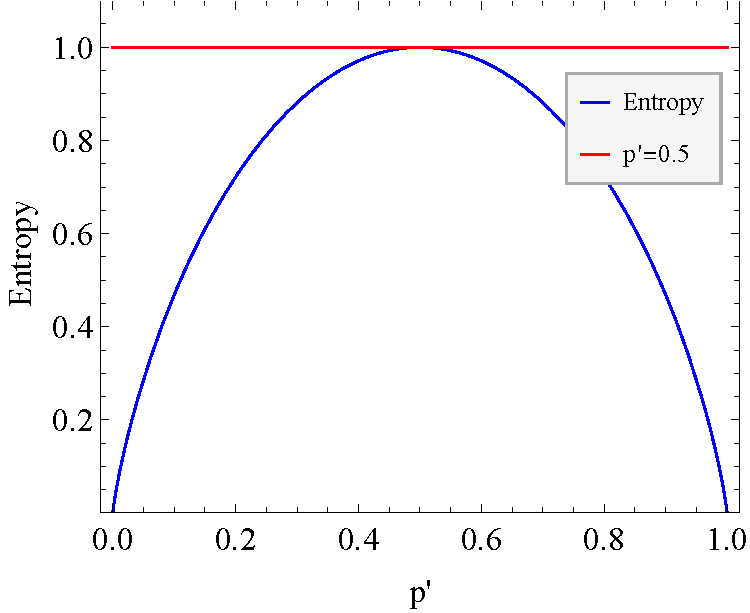
\includegraphics[width=\figwidth]{entropy}
\postfig\precaption
\caption{Information entropy of a BF}
\postcaption
\label{fig:entropy}
\end{figure}

\presub \subsection{Relation Between False Positive Probability and Information Entropy} \postsub
%
We now show the relation between the false positive probability and information entropy. 
%
We first present a lemma and some definitions.

\noindent\textbf{Lemma I:} Given a BF, suppose $n$ and $k$ keep unchanged, when $m$ becomes larger, the FP probability gets smaller.

\begin{proof}
When $n$ and $k$ are fixed, for larger $m$, the probability of each bit being 1 in the BF becomes smaller, \ie, $p'$ becomes smaller; thus, the FP probability gets smaller.
\end{proof}

%%
\noindent\textbf{Definition I:} \textit{Bloom filter variable.} The false positive rate of Bloom filters is determined by $m$, $n$, and $k$. For different $n$ elements, the $m$-bit string varies. Thus, when the values of $m$, $n$, $k$ are given, the $m$-bit string is a \textit{random variable}. When the $n$ elements are given, the $m$-bit string is a random variable instance. Therefore, when the values of $m$, $n$, $k$ are given, we call it a Bloom Filter Variable (BFR). Since it is a random variable, we can compute its information entropy.

\noindent\textbf{Definition II:} \textit{Equivalent Bloom filter variables.} Given two Bloom filters variables $v_1$ and $v_2$, for the same $n$ elements, there are a pair of BFR instances. Given a set with $n$ elements, if these pairs of BFR instances always report the same result: true or false for any input element, we say $v_1$ and $v_2$ are equivalent.

\noindent\textbf{Theorem I:} Given a Bloom filter \textit{variable} $v_1$ with parameters $m$, $n$, and $k$, if its information entropy is not at the maximum, there must exist a smaller equivalent Bloom filter variable $v_2$ with parameters $m'$, $n$ and $k$, where $m'<m$.

\begin{proof}
For $v_1$, the parameters are $m$, $n$, $k$. 
%
Suppose its $k$ hash functions are $h_1(\cdot), h_2(\cdot), \ldots, h_k(\cdot)$.
%
Since the assumption is that the information entropy of $v_1$ is not at the maximum, according to the property of information entropy, $v_1$ can be compressed \textit{without information loss}. 
%
After compression, suppose the new random variable has a length of $m' (m' < m)$, we name it $v_2$.
%
Note that during the compression, the information value $m*E$ keeps unchanged, while $E's$ maximum value is 1; thus, the length of the compressed message has a minimum value.
%
Here $v_1$ and $v_2$ are two variables consisting of bits, and we can treat them as two integer variables. 
%
We use $In(v_1)$ and  $In(v_2)$ to represent the integer value of $v_1$ and $v_2$.
%
Furthermore, we use $|In(v_1)|$ represents the length of $v_1$, then we have  $|In(v_1)|=m$, $|In(v_2)|=m'$.
%
Because we compress $v_1$ and get $v_2$, this can be regarded as a function $g(\cdot)$. 
%
In other words, $g(In(v_1))=In(v_2)$. 
%
We can also obtain $v_1$ by equation $In(v_1)=g^{-1}(In(v_2))$.

At this stage, we consider the new Bloom filter variable $v_2$, the parameters are $m'$, $n$, and $k$.
%
Note that we use $k$ \texttt{different} hash functions, and the $k$ hash functions are
%
\begin{equation}
\begin{aligned}
&g^{-1}(In(v_2))\ll h_1(y) \gg (|g^{-1}(In(v_2))|-h_1(y)-1), \\
&g^{-1}(In(v_2))\ll h_2(y) \gg (|g^{-1}(In(v_2))|-h_2(y)-1), \\
& \ldots \\
&g^{-1}(In(v_2))\ll h_k(y) \gg (|g^{-1}(In(v_2))|-h_k(y)-1)
\end{aligned}
\label{equ:g(k)}
\end{equation}
%
Where `$\ll$' means left shift and `$\gg$' means right shift.

Given an input element $y$, we can compute the above $k$ values only using $v_2$ and $h_i(\cdot)$ without $v_1$.
%
Then we need to prove that for any incoming element $y$, $v_2$ reports the same $k$-bit value.
%
With formula \ref{equ:g(k)}, we use equation $v_1=g^{-1}(In(v_2))$ and $m=|g^{-1}(In(v_2))|$.
%
These $k$ hash functions are simplified as
%
\begin{equation}
\begin{aligned}
&v_1\ll h_1(y) \gg (m-h_1(y)-1), \\
&v_1\ll h_2(y) \gg (m-h_2(y)-1), \\
& \ldots \\
&v_1\ll h_k(y) \gg (m-h_k(y)-1)
\end{aligned}
\label{equ:g(k):simple}
\end{equation}
%
Here $1\leqslant i\leqslant k$ and $0\leqslant h_i(y)\leqslant m-1$.
%
Here $v_1\ll h_i(y) \gg (m-h_i(y)-1)$ actually means the value of $h_i(y)$-th bit of $v_1$.
%
This is the same as the $k$ hash functions as $v_1$. 
%
Therefore, $v_1$ and $v_2$ are equivalent.
\end{proof}

\noindent\textbf{Theorem II:} Given a Bloom filter variable,  \textit{if and only if} its information entropy is at the maximum, its FP probability is at the minimum.

\begin{proof}
%
First, we prove that if the FP probability is at the minimum, then its information entropy must be at the maximum. 
%
Given a Bloom filter variable $v_1$ with parameters $m$, $n$, $k$. 
%
Since the assumption is that the information entropy of $v_1$ is not at the maximum, according to Theorem I, there exists a smaller Bloom filter variable $v_2$ with parameters $m'$, $n$, $k$. 
%
Since $v_2$ and $v_1$ are equivalent, their FP probabilities are the same, we name it $f$.
%
At this stage, we enlarge the size of $v_2$ a little from $m'$ to $m''$, where $m'<m''<m$. 
%
According to Lemma I, we know the FP probability of $v_2$ becomes smaller than $f$. 
%
This means that for $v_1$, there exists a BF variable with a smaller size and a smaller FP probability.
%
Therefore, the FP probability of $v_1$ is not at the minimum.
%
This means that if its information entropy is not at the maximum, then the FP probability is definitely not at the minimum. 
%
The contrapositive is that if the FP probability is at the minimum, then its information entropy must be at the maximum.

%%
Second, we prove that if its information entropy is at the maximum, the FP probability is at the minimum.
%
Given a Bloom filter variable $v_1$ with parameters $m$, $n$, $k$. 
%
Since the assumption is that the FP probability of $v_1$ is not at the maximum, there exists an optimal Bloom filter variable $v_0$ with parameters $m$, $n$, $k'$, where $k'\neq k$. 
%
According to $\leftarrow$, the information entropy of $v_0$ is at the maximum. 
%
According to Eq. \ref{equ:entropyBF} and Figure \ref{fig:entropy}, the $p'$ of $v_0$ is 0.5 whereas the $p'$ of $v_1$ is not because they have different value of $k$. 
%
Therefore, the information entropy of BF$_1$ is not at the maximum.
%
This means if the FP probability is not at the minimum, its information entropy must be not at the maximum. 
%
The contrapositive is that if its information entropy is at the maximum, the FP probability is at the minimum.
\end{proof}

\presub \subsection{Computing the Optimal k} \postsub
\label{optk}
%
According to Theorem II, when the information entropy of the Bloom filter variable is at the maximum, the FP probability is at the minimum.
%
Recalling the definition of $p'$ in Eq. \ref{p'form}, one can use this interpretation to find $k^*$, \ie, the optimal number of hash functions. 
%
From Figure \ref{fig:entropy}, we know that when $p'$ is 0.5, $E$ reaches the maximum value 1. By setting the value of $p'$ to 0.5, we have
%
\begin{equation}
p'=\left(1-\frac{1}{m}\right)^{k^* n}=0.5
\label{equ:p=0.5}
\end{equation}
%
Further, we have:
\begin{equation}
\label{equ:mykform}
k^*=-\dfrac{\ln 2}{n} / \ln\left(1-\dfrac{1}{m}\right)
\end{equation}
%
This formula is very close to the formula of $k^*$ obtained by Bloom. 
%
When $x$ is very small, $\ln(1+x)\approx x$, and therefore $-1/\ln(1-\dfrac{1}{m}) \approx m$, resulting the same term as in Eq. \ref{eq:kopt}.

\noindent\textbf{Theorem III:} Given any BF variable, when $m$ and $n$ are fixed, the FP probability $f$ is a function of $k$, we represent it $f(k)$. Then $f(k)$ is a \textit{convex function}, which has only one minimum value.

\begin{proof}
Given a Bloom filter variable $v_1$ with parameters $m$, $n$, $k_1$, its entropy is $E_1$.
%
Given another Bloom filter variable $v_2$ with parameters $m$, $n$, $k_2$, its entropy is $E_2$.
%
(1) For any $k_1<k_2\leqslant k^*$, according to Eq. \ref{p'form}, Eq. \ref{equ:entropyBF} and Figure \ref{fig:entropy}, we known $p'_1<p'_2\leqslant 0.5$.
%
We compress $v_1$ to $v_3$ with parameters $m_3$, $n$, $k_1$. 
%
To make $v_3$'s entropy equal to $E_2$, $m_3$ should be $mE_1/E_2$. 
%
In this case, the entropy of $v_3$ is equal to that of $v_2$. 
%
When the entropy of BF variables is less than 0.5, the same entropy leads to the same $p'$. 
%
In other words, $p'_3=p'_2$. 
%
Because $v_2$ has more hash functions ($k_2>k_1$), the FP probability of $v_2$ is smaller than that of $v_3$. 
%
While $v_3$ and $v_1$ have the same FP probability, therefore, the FP probability of $v_2$ is smaller than that of $v_1$.
%
In other words, for any $k (k<k^*)$ increasing, the FP probability of BFs decreases.
%
(2) For any $k^*\leqslant k_1<k_2$, according to Eq. \ref{p'form}, Eq. \ref{equ:entropyBF} and Figure \ref{fig:entropy}, we known $p'_1>p'_2\geqslant 0.5$.
%
Using the similar derivation, we can derive that the FP probability of $v_2$ is larger than that of $v_1$.
%
According to the above two cases, we know that given any BF variable, when $m$ and $n$ are fixed, the FP probability $f$ is a function of $k$, we represent it $f(k)$.  
%
So $f(k)$ is a \textit{convex function}.
\end{proof}
\presec \section{Asymptotic Form of the FP Probability} \postsec \label{sec:limitf}
%
In this section, we derive a new approach to computing the asymptotic form for the FP probability of BFs. 
%
The new derivation is based on \textit{partitioned Bloom Filters} (pBF) that are used frequently to carry out parallel queries. 
%
Its underpinning principle is simple: the BF is divided into $k$ even partitions, and each hash function only acts on one of the partitions, respectively.
%
The probability that one bit of the BF array remains 0 after inserting $n$ elements in the BF becomes the following as now each hash maps into $\frac{m}{k}$ separate bits.
%
\begin{equation}
p'_{partition} = \left( 1-\dfrac{k}{m} \right)^n
\label{equ:p'pBF}
\end{equation}

It is intuitive that the FP probability of partitioned BF is a little bigger than that of BF. 
%
Unfortunately, there is no strict proof. 
%
Here we show one proof method, which is based on the following Lemma. 

\vspace{0.05in}
\noindent\textbf{Lemma II:} For $m > 1 \;\;,   k >1, \;\; n > 1, \: m>k$,
\begin{equation}
\label{theorem1}
\left( 1-\dfrac{k}{m} \right)  ^n <
\left( 1-\dfrac{1}{m} \right)  ^{kn}
\end{equation}

\begin{proof}
Note that when $m$ is large, the left expression approximates to the right one. Below we give the derivation details.
%
Let $g(k)=( 1-\frac{1}{m} )  ^k- ( 1-\frac{k}{m} )$. 
%
For $m>1$ and $k>1$, $g(k)$ is a continuous and derivable function, and we can obtain the following inequality in terms of its derivative:
%
\begin{equation}
\begin{aligned}
%g'(k)=k\left( 1- \dfrac{1}{m}\right) ^{k-1} +\dfrac{1}{m}
g'(k) %&=\left( 1- \dfrac{1}{m}\right)^k \ln\left(1-\dfrac{1}{m}\right)+\dfrac{1}{m} \\
> \left( 1- \dfrac{1}{m}\right)\ln\left(1-\dfrac{1}{m}\right)+\dfrac{1}{m}
\end{aligned}
\end{equation}
%
Let $f(m)=\left( 1- \dfrac{1}{m}\right)\ln\left(1-\dfrac{1}{m}\right)+\dfrac{1}{m}$.
%
Then $f'(m) = \dfrac{1}{m^2} \ln\left(1-\dfrac{1}{m}\right)< 0$, which means that the function $f(m)$ is strictly decreasing.
%
When $m$ goes to infinity, we have $\lim\limits_{m \to \infty}  f(m) =  0$. 
%
Therefore, we know that $f(m) \geqslant 0$, and $g'(k) > f(m) \geqslant 0$, which means that the function $g(k)$ is strictly increasing.
%
Thus, we have
%

\begin{equation}
\left( 1-\dfrac{k}{m} \right) ^n   <
\left( 1-\dfrac{1}{m} \right)  ^{kn}
\end{equation}
\end{proof}

The above lemma shows that $p'_{partition} < p'_{true}$ or equivalently $1-p'_{partition} > 1-p'_{true}$.
%
Thus, we know that with the same parameters, the FP probability of the pBF will be larger than that of the standard BF $f_{true}$, \ie, $f_{partition} > f_{true}$. 
%
In addition, Bose’s bounds in Eq. \ref{fBound} state that the precise value of FP probability for a BF $f_{true}$ is larger than $f_{bloom}$, \ie, $f_{true} > f_{bloom}$. 
%
Therefore, we have the following upper and lower bounds:

\begin{equation}
\label{bigbig}
f_{partition} > f_{true} > f_{bloom}
\end{equation}

For a partitioned BF, the probability that one bit of the array is still 0 $p'$ is shown in Eq. \ref{equ:p'pBF}.
%
Different from standard Bloom Filters, for a partitioned Bloom Filter, the event $E(h_1=1),E(h_2=1),E(h_3=1),...,E(h_{i-1}=1)$ is independent of the event $E(h_{i-1}=1)$, where $E(h_{i-1}=1)$ means that the event that the position of $h_{i-1}(x)$ is 1 because each hash function is responsible for one partition, and has no impact on each other. 
%
Therefore, we have
%
\begin{equation}
f_{partition}=(1-p'_{partition})^k=\left( 1- \left( 1-\dfrac{k}{m} \right)^n \right) ^k
\end{equation}
Then the formula~\ref{bigbig} becomes

\begin{equation}
\label{bounds}
\left( 1- \left( 1-\dfrac{k}{m} \right)^n \right) ^k > f_{true} > \left( 1- \left( 1-\dfrac{1}{m} \right)^{nk} \right) ^k
\end{equation}

Then we use the well known limit formula:
\begin{equation}
\lim\limits_{x \to \infty} \left( 1-\dfrac{1}{x}\right) ^{-x} = e
\end{equation}

%%
Asymptotically, when $m$ becomes large, we already know that $f_{bloom}$ converges to the term in Eq. \ref{fBloom}. 
%
Nevertheless, the upper bound has also an asymptotic behaviour as the following, which is the same term as the lower bound limit. 
%
\begin{equation}
\label{flim}
\lim\limits_{m \to \infty} \left(1-\left(1-\frac{1}{m}\right)^{nk}\right)^k = \left(1-e^{-nk/m}\right)^k 
\end{equation}
%
Through the Sandwich Theorem (also known as squeeze theorem) we obtain the following equation, which is similarly to Christensen and Bose:
\begin{equation}
\label{flimtrue}
\lim\limits_{m \to \infty}  f_{true} =  \left(1-e^{-nk/m}\right)^k 
\end{equation}

This means that when $m$ is large, the Bloom's formula can be used with negligible error. 
%
However, we still need to evaluate what means \textit{$m$ being large}. 
%
We will do this by comparing the two bounds we have in hand: the one from Bose and the one we derived in this paper.
%
We show in Figure~\ref{fig:uplowbound} that the two upper bounds along with the lower bound obtained for $k=7$  and $m=10n$ as a function of $n$, the number of elements inserted in the BF.
%
As can be seen, the upper bound derived in this paper and the lower bound $f_{bloom}$ converge relatively fast for $n=9$, while the upper bound derived by Bose has a much slower convergence. 
%
We can see this better by looking at the behavior of the bounds error ratio $\beta$, defined as $\beta=\frac{upper\ bound - lower\ bound}{lower\ bound}$, for the two bounds in Figure \ref{fig:ratio}.

\begin{figure}[t]
\centering
\prefig
\vspace{-0.1in}
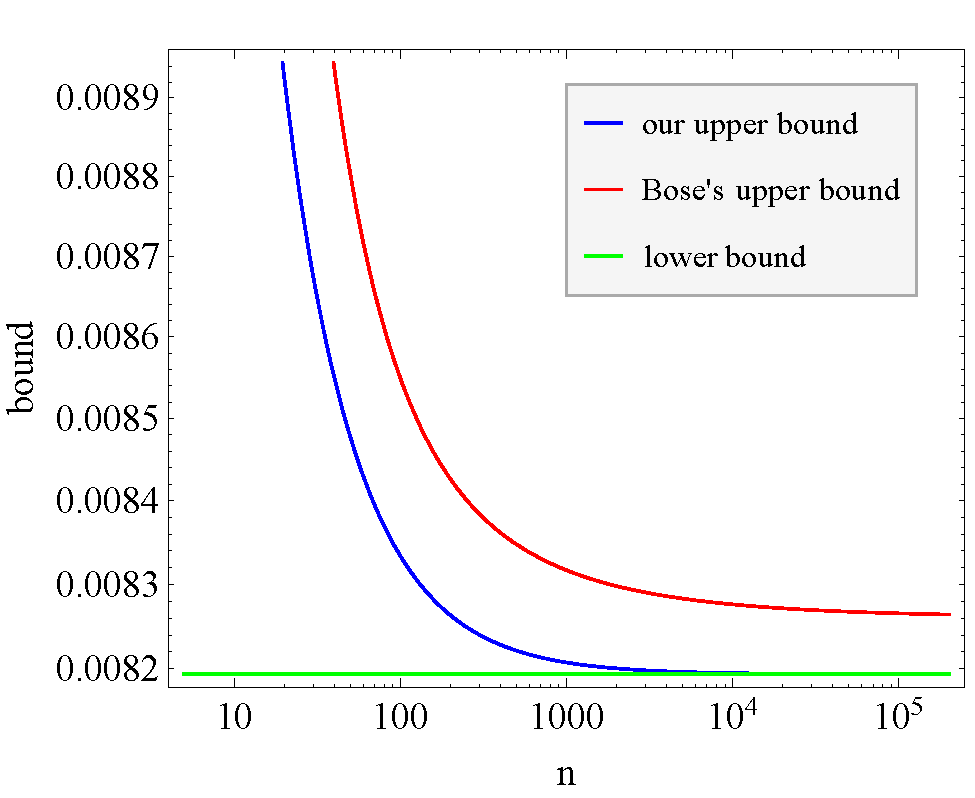
\includegraphics[width=\figwidth]{LogLog_lowerUpper}
\postfig\precaption
\vspace{0.1in}
\caption{Upper and lower bound for $f_{true}$ for $k=7$ and $m=10n$.} 
\postcaption
\vspace{0.1in}
\label{fig:uplowbound}
\end{figure}

\begin{figure}[t]
\centering
\prefig
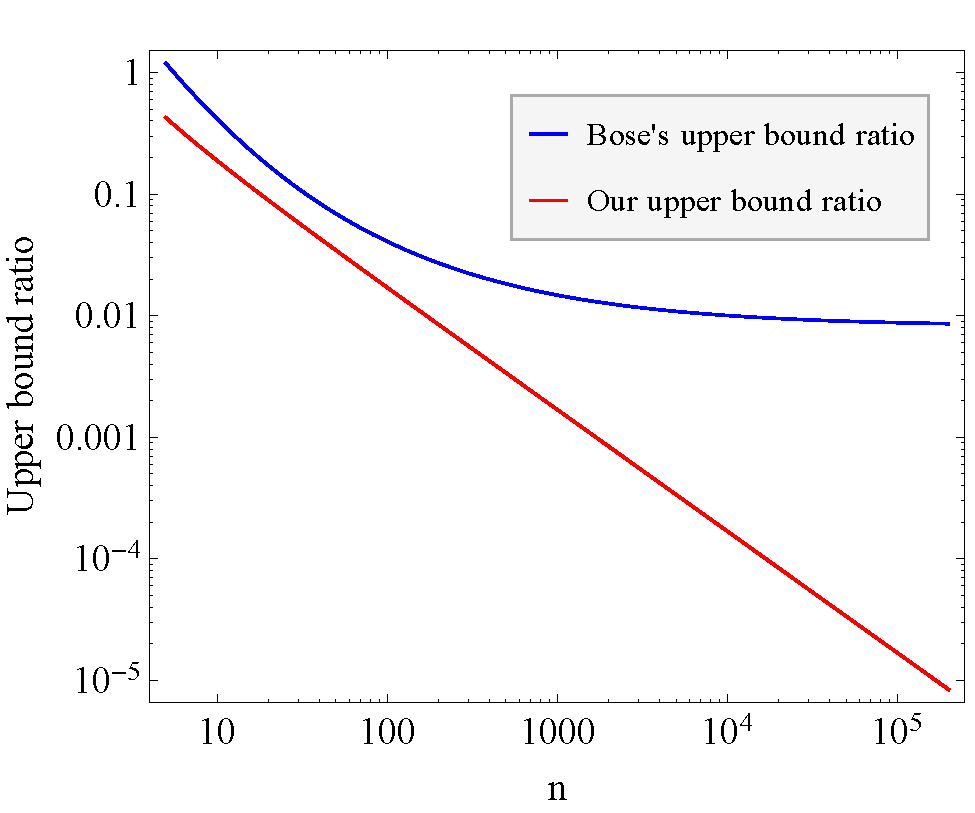
\includegraphics[width=\figwidth]{LogLog_ratio}
\postfig\precaption\vspace{0.1in}
\caption{Bounds error ratio for Bose's bound and the bound derived in this paper for $k=7$ and $m=10n$. } 
\postcaption
\vspace{0.1in}
\label{fig:ratio}
\end{figure}

As can be seen, the gap between our derived upper bound and $f_{bloom}$ is decreasing polynomially at a constant speed, while Bose's bound has a lower speed of convergence. In order to extend this observation, we show in Figure \ref{fig:ratiok} the evolution of the bounds error ratio for a BF with $m=10000$, $n=1000$ and varying $k$. 

\begin{figure}[htbp]
\centering
\prefig
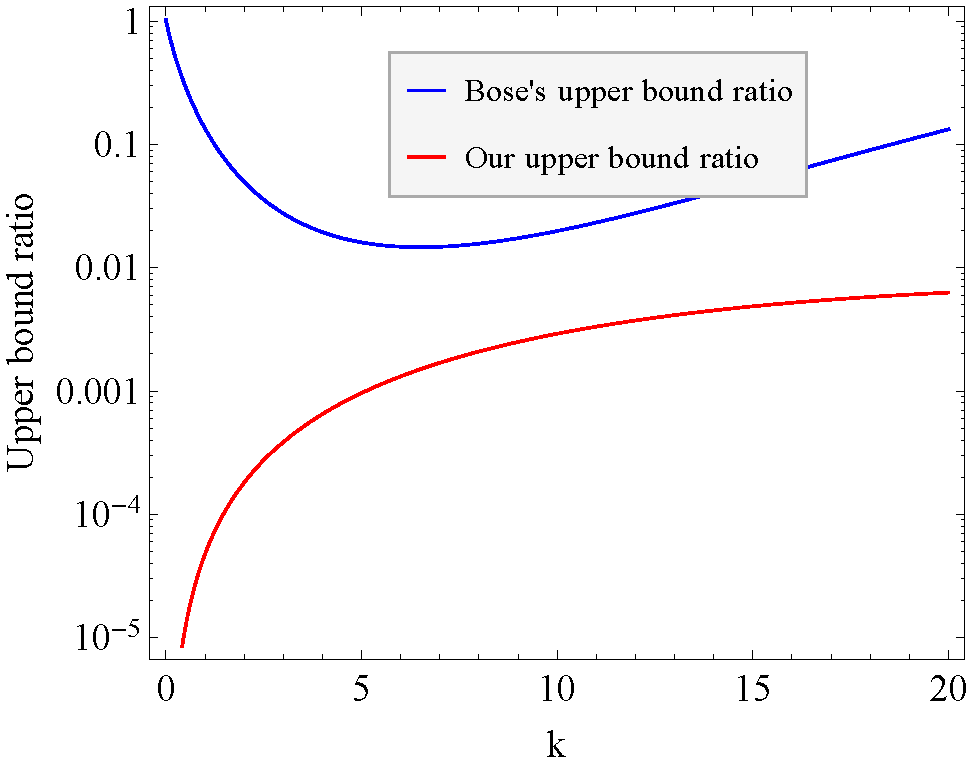
\includegraphics[width=\figwidth]{ratioLog_k}
\postfig\precaption\vspace{0.10in}
\caption{Bounds error ratio for Bose's bound and the bound derived in this paper for $m=10000$, $n=1000$ and varying $k$.}  
\postcaption
\vspace{0.1in}
\label{fig:ratiok}
\end{figure}

As expected, error involved with using $f_{bloom}$ increases with the number of hash functions $k$ increases. 
%
However, it can be seen that the convergence behavior of the bounds derived in this paper is much better than the one obtained by Bose. 

\begin{comment}
The calculation of the correct rate of the counting Bloom filter \cite{cbf}, $\mathcal{C}_r$, can benefit from our derivation about the false positive probability of standard Bloom filter. 
%
The counting Bloom filter (CBF), one variant of standard Bloom filter, replaces each bit with one counter, supporting estimating the frequency of each inserted item. 
%
In CBF, the over-estimation of an inserted item is equivalent to one false positive in standard Bloom filter. 
%
Therefore, we have: 
\begin{equation}
\mathcal{C}_r = 1 - f_{true}
\end{equation}
%
Applying equation \ref{bounds}, we can get the upper and lower bounds of the $\mathcal{C}_r$ of CBF. 
\end{comment}

%\presec
\section{Experimental Results} \postsec
\label{sec:evaluation}
%In this section, we evalute the 

The goal of this section is to validate the accuracy and correctness of our proposed bound and formula.
In this section, we first validate the formula $f_{bloom}$, and then validate our proposed formula of optimal $k$ -- equation \ref{equ:mykform}.

\presub
\subsection{Experimental Setup} \postsub
In order to evaluate experimentally the FP probability of a set of entries, we wrote a C++ program to generate a large set of unique entries with 20 characters in each. 
%
It takes around 1 hour on an Intel(R) Core(TM) i7-920 with a 4-core computer working at 2.67GHz to generate 100M unique entries and more than 3 hours to get 300M entries which occupy more than 6GB memory. 
%
These two sets are used to evaluate FP probability and optimal values of $k$.
%In place of trying to find hash functions with low complexity we rather use hash functions known to be uniform. For this purpose, we collect 26 hash functions mainly from website \cite{...}, 
We collect 20 hash functions, mainly from \cite{hashfuncssigcommccr}, and the name of hash functions are shown in Table 
\ref{table:hashfunction}. We choose different hash functions for the experiments several times, and the experimental results show little differences and thus we only show the experimental results when using the first $k$ hash functions.

%a set of hashing function based on 26 basic hash functions and we build the needed hash functions from this universal hash function.


%TABLE III
%COLLECTED HASH FUNCTIONS AND THEIR NUMBER IN THIS PAPER
%APHash BKDR BOB CRC32 DEKHash
%h1 h2 h3 h4 h5
%DJBHash FNV32 Hsieh JSHash OCaml
%h6 h7 h8 h9 h10
%OAAT PJWHash RSHash SBOX SDBM
%h11 h12 h13 h14 h15
%Simple SML STL MD5 SHA-1
%h16 h17 h18 h19 h20


\begin{table} [htbp]
\vspace{0in}
\caption{Hash functions used in our experiments.}
\centering
\label{table:hashfunction}
\begin{tabular}{| l | l | l | l | l |}
\hline 1: APHash  & 2: BKDR  & 3: BOB  & 4: CRC32 & 5: DEKHash \\
\hline 6: DJBHash & 7: FNV32 & 8: Hsieh & 9: JSHash & 10: OCaml \\
\hline 11: OAAT & 12: PJWHash & 13: RSHash &14: SBOX &15: SDBM \\
\hline 16: Simple &17: SML & 18: STL & 19: MD5 &20: SHA-1 \\
\hline
\end{tabular}
\end{table}





\presub
\subsection{False Positive Probability Test} \postsub

\begin{table}[htbp]
\vspace{0in}
	\centering\caption{False positive probability in theory and simulation.}
\vspace{0in}
	\begin{tabular}{l l l l l}
		\hline
		k   &	\# of FP	&	FP from $f_{bloom}$	&	FP of simulation	&	Error ratio	(\%)\\
		\hline
		2	&	24814826	&	0.25003480 	&	0.24814830 	&	-0.7545290 	\\
		4	&	6263312	&	0.06250841 	&	0.06263312 	&	0.1995030 	\\
		6	&	1565056	&	0.01562703 	&	0.01565056 	&	0.1505790 	\\
		8	&	392198	&	0.00390674 	&	0.00392198 	&	0.3901310 	\\
		10	&	95314	&	0.00097668 	&	0.00095314 	&	-2.4102060 	\\
		12	&	24946	&	0.00024417 	&	0.00024946 	&	2.1670100 	\\
		14	&	6166	&	0.00006104 	&	0.00006166 	&	1.0125530 	\\
		16	&	1528	&	0.00001526 	&	0.00001528 	&	0.1283920 	\\
		\hline
	\end{tabular}
	\label{table:fp:theory:sim}
\end{table}


\begin{figure*}[htbp]
 	\begin{minipage}{0.28\linewidth}
 		\centerline{\includegraphics[width=6.2cm]{fperrork4}}
 		\centerline{(a) k=4}
 	\end{minipage}
 	\hfill
 	\begin{minipage}{0.28\linewidth}
 		\centerline{\includegraphics[width=5.8cm]{fperrork5}}
 		\centerline{(b) k=5}
 	\end{minipage}
 	\hfill
 	\begin{minipage}{0.28\linewidth}
 		\centerline{\includegraphics[width=5.8cm]{fperrork6}}
 		\centerline{(c) k=6}
 	\end{minipage}
 	\caption{FP probability error ratio vs. \# of queries with different $k$.}  \vspace{0in}
 	\label{fig:error:ratio}
 \end{figure*}

 \begin{figure*}[htbp]
 	\begin{minipage}{0.28\linewidth}
 		\centerline{\includegraphics[width=6.2cm]{FPtheorysimk4}}
 		\centerline{(a) k=4}
 	\end{minipage}
 	\hfill
 	\begin{minipage}{0.28\linewidth}
 		\centerline{\includegraphics[width=5.8cm]{FPtheorysimk5}}
 		\centerline{(b) k=5}
 	\end{minipage}
 	\hfill
 	\begin{minipage}{0.28\linewidth}
 		\centerline{\includegraphics[width=5.8cm]{FPtheorysimk6}}
 		\centerline{(c) k=6}
 	\end{minipage}
 	\caption{FP probability error vs. \# of queries with different $k$.}  \vspace{-0.07in}
 	\label{fig:error:abso}
 \end{figure*}
 
  \begin{figure*}[htbp]
  	\begin{minipage}{0.28\linewidth}
  		\centerline{\includegraphics[width=6.2cm]{NotAcck4}}
  		\centerline{(a) k=4}
  	\end{minipage}
  	\hfill
  	\begin{minipage}{0.28\linewidth}
  		\centerline{\includegraphics[width=5.8cm]{NotAcck5}}
  		\centerline{(b) k=5}
  	\end{minipage}
  	\hfill
  	\begin{minipage}{0.28\linewidth}
  		\centerline{\includegraphics[width=5.8cm]{NotAcck6}}
  		\centerline{(c) k=6}
  	\end{minipage}
  	\caption{FP probability error vs. \# of queries with independent queries.} \vspace{-0.07in}
  	\label{fig:error:notAcc}
  \end{figure*}
 
  
  \begin{figure*}[htbp]
  	\begin{minipage}{0.28\linewidth}
  		\centerline{\includegraphics[width=6.2cm]{m12n8k}}
  		\centerline{(a) n=8,000}
  	\end{minipage}
  	\hfill
  	\begin{minipage}{0.28\linewidth}
  		\centerline{\includegraphics[width=5.8cm]{m12n10k}}
  		\centerline{(b) n=10,000}
  	\end{minipage}
  	\hfill
  	\begin{minipage}{0.28\linewidth}
  		\centerline{\includegraphics[width=5.8cm]{m12n12k}}
  		\centerline{(c) n=12,000}
  	\end{minipage}
  	\caption{Variation of FP probability as a function of the number of hash functions $k$ for $m=100,000$ and different number of inserted entries $n$} \vspace{0in}
  	\label{fig:bestk}
  \end{figure*}
  
  


%ShBFM calculated in Equation (1) using our experimental
%results. Then we compare ShBFM with BF and 1MemBF
%[14], which represents the prior scheme for answering mem-
%bership queries, in terms of FPR, the number of memory
%accesses, and query processing speed.




\subsubsection{Basic Test} \textit{Our experimental results show that the error ratio shows that the experimental results of FP probability follow the predictions of $f_{bloom}$ very well.}
In this experiment, we use the 100M-entries file described above. Each round of experiments is done with a given value of $k$ chosen as an even number from 2 to 16.
We insert the first 5000 ($n$ = 5000) elements into the Standard Bloom Filter (SBF), and then calculate the optimal $m$ according to the formula~\ref{equ:mykform}, and then get:
%\begin{equation}
%\label{formulaM}
%m=\dfrac{k*n}{ln2}
%\end{equation}
\begin{equation}
\label{formulaM}
m=\dfrac{1}{1-2^{-\dfrac{1}{kn}}}
\end{equation}
In order to evaluate the FP probability, we query 100M elements from the BF we built, and the query results are shown in Table \ref{table:fp:theory:sim}.
%
We show experimental results of FP probability of BF as well as the FP probability using the formula of $f_{bloom}$.
%also in the table along with the empirically estimated FP probability the one predicted using the $f_{bloom}$ as well as the error ratio between these two rates.
It can be seen that as $k$ increases from 2 to 16, the number of false positives decreases from 24814826 to 1528 and the error ratio is 2.41\% at most.




 \subsubsection{Error ratio vs. Querying number}

 
  
  
 We build the same SBF as described previously and use the same 100M-traffic file. We run experiments when $k$ is 4, 5, and 6, respectively. $n$ is still 5000, and $m$ is calculated to be the optimal number according to formula \ref{formulaM}. We query 1M up to 100M elements and calculate the error ratio when every next 1M elements are queried.
 %We compute the FP probability using the accumulated sum of the FP number, which also contains the ones counted before. So we can get 100 error ratio spots. That means the $100th$ result of FP number contains all the previous ones.


The results are shown in Figure \ref{fig:error:ratio}. It shows that at the very beginning, the error ratio is much bigger and also with drastic fluctuation. The more elements we query, the stabilizer the error ratio will be.
%It is because when the number of query elements is large, the FP number will be bigger and the results will be more accurate.
When the number of false positives in a test is small, the test results can hardly be reliable. In our test, the smallest number of false positives is 15,820, which is the first spot in Figure \ref{fig:error:ratio}c, when $k$ is 6 and query number is 1M.
All in all, the error ratio is actually so small that it can be ignored. They are ranging from -0.533\% to +0.356\% when $k=4$, ranging from +0.188\% to +0.699\% when $k=5$, and ranging from -0.138\% to +1.235\% when $k=6$.



 To give a more intuitive result, we plot Figure \ref{fig:error:abso}. The blue line is the theoretical FP probability, while the other curve is the evaluated FP probability (defined as FP number/total query number). That error ratio stabilizes with the increase of the querying number still holds.


To give a whole picture, we carry out another experiment. In this experiment, we query the first $n$ elements and sum up the FP number. And then, we pick up the latter $n$ elements and also get the FP number. These two groups of elements are totally different without duplicate elements across the groups. Thus, we query up to $100*n$ elements and get 100 spots. The 100M-element traffic file is not large enough for this experiment, so we use the 300M-element traffic file which contains more than 300M elements we described in the experimental setup section.

As shown in Figure \ref{fig:error:notAcc}, the smallest number of false positives is 1,075, which is still in the first spot in Figure \ref{fig:error:notAcc}c, when $k$ is 6 and this time query number is 68,712. Although it is smaller than the previous accumulated experimental results, it is still bigger than 1,000, so the result is reasonable. By the way, the 100th query number is $100*68712=6,871,200$ and the number of FP is 109,713, which is large enough.

 It can be seen from Figure \ref{fig:error:notAcc}, the error ratios fluctuate drastically at the beginning and quickly converge to a small range. And also, the error ratios are very small ranging from -0.812\% to +1.500\% when $k=4$, ranging from -3.559\% to +1.284\% when $k=5$, and ranging from +0.115\% to +5.581\% when $k=6$.

\presub
\subsection{Optimal $k$ Formula Validation} \postsub


\textit{Our experimental results show that our proposed formula of optimal $k$ is accurate.}
In this experiment, we validate that the formula Eq. \ref{equ:mykform} derived for $k^*$, gives a value minimizing the FP probability. For this purpose, we create large Bloom filters with $m=100,000$ and with different $k$ varying from 2 to 16,  and then insert $n=8000$, $10000$, and $12000$ entries into it, respectively. We use the same 100M-entries to evaluate the FP probability. We show the results in Figure \ref{fig:bestk}. We also show the value of FP probability derive using the formula $f_{bloom}$.


It can be seen in the figure \ref{fig:bestk} for the given value of $m$, $n$, and $k$, the experimental results and the theoretical values of FP probability match well. Moreover, when using formula in Eq. \ref{equ:mykform}, on the third scenario that is $n=12,000$, one can derive an optimal value of $k^*=6$. As shown in Figure \ref{fig:bestk}, it can be seen that this is indeed the value minimizing the FP probability to be 1.816\%. Similar observations are made for $n=8000$ and $10,000$.

% \begin{figure*}[htbp]
 %	\begin{minipage}{0.28\linewidth}
 %		\centerline{\includegraphics[width=6.2cm]{PCQpsk4}}
 %		\centerline{(a) k=4}
 %	\end{minipage}
 %	\hfill
 %	\begin{minipage}{0.28\linewidth}
 %		\centerline{\includegraphics[width=5.8cm]{PCQpsk6}}
 %		\centerline{(b) k=6}
 %	\end{minipage}
 %	\hfill
 %	\begin{minipage}{0.28\linewidth}
 %		\centerline{\includegraphics[width=5.8cm]{PCQpsk8}}
 %		\centerline{(c) k=8}
 %	\end{minipage}
 %	\caption{Query speed (Qps) with different traffic.}
 %	\label{fig:PC:QPS}
 %\end{figure*}

% \begin{figure*}[htbp]
 %	\begin{minipage}{0.28\linewidth}
 %		\centerline{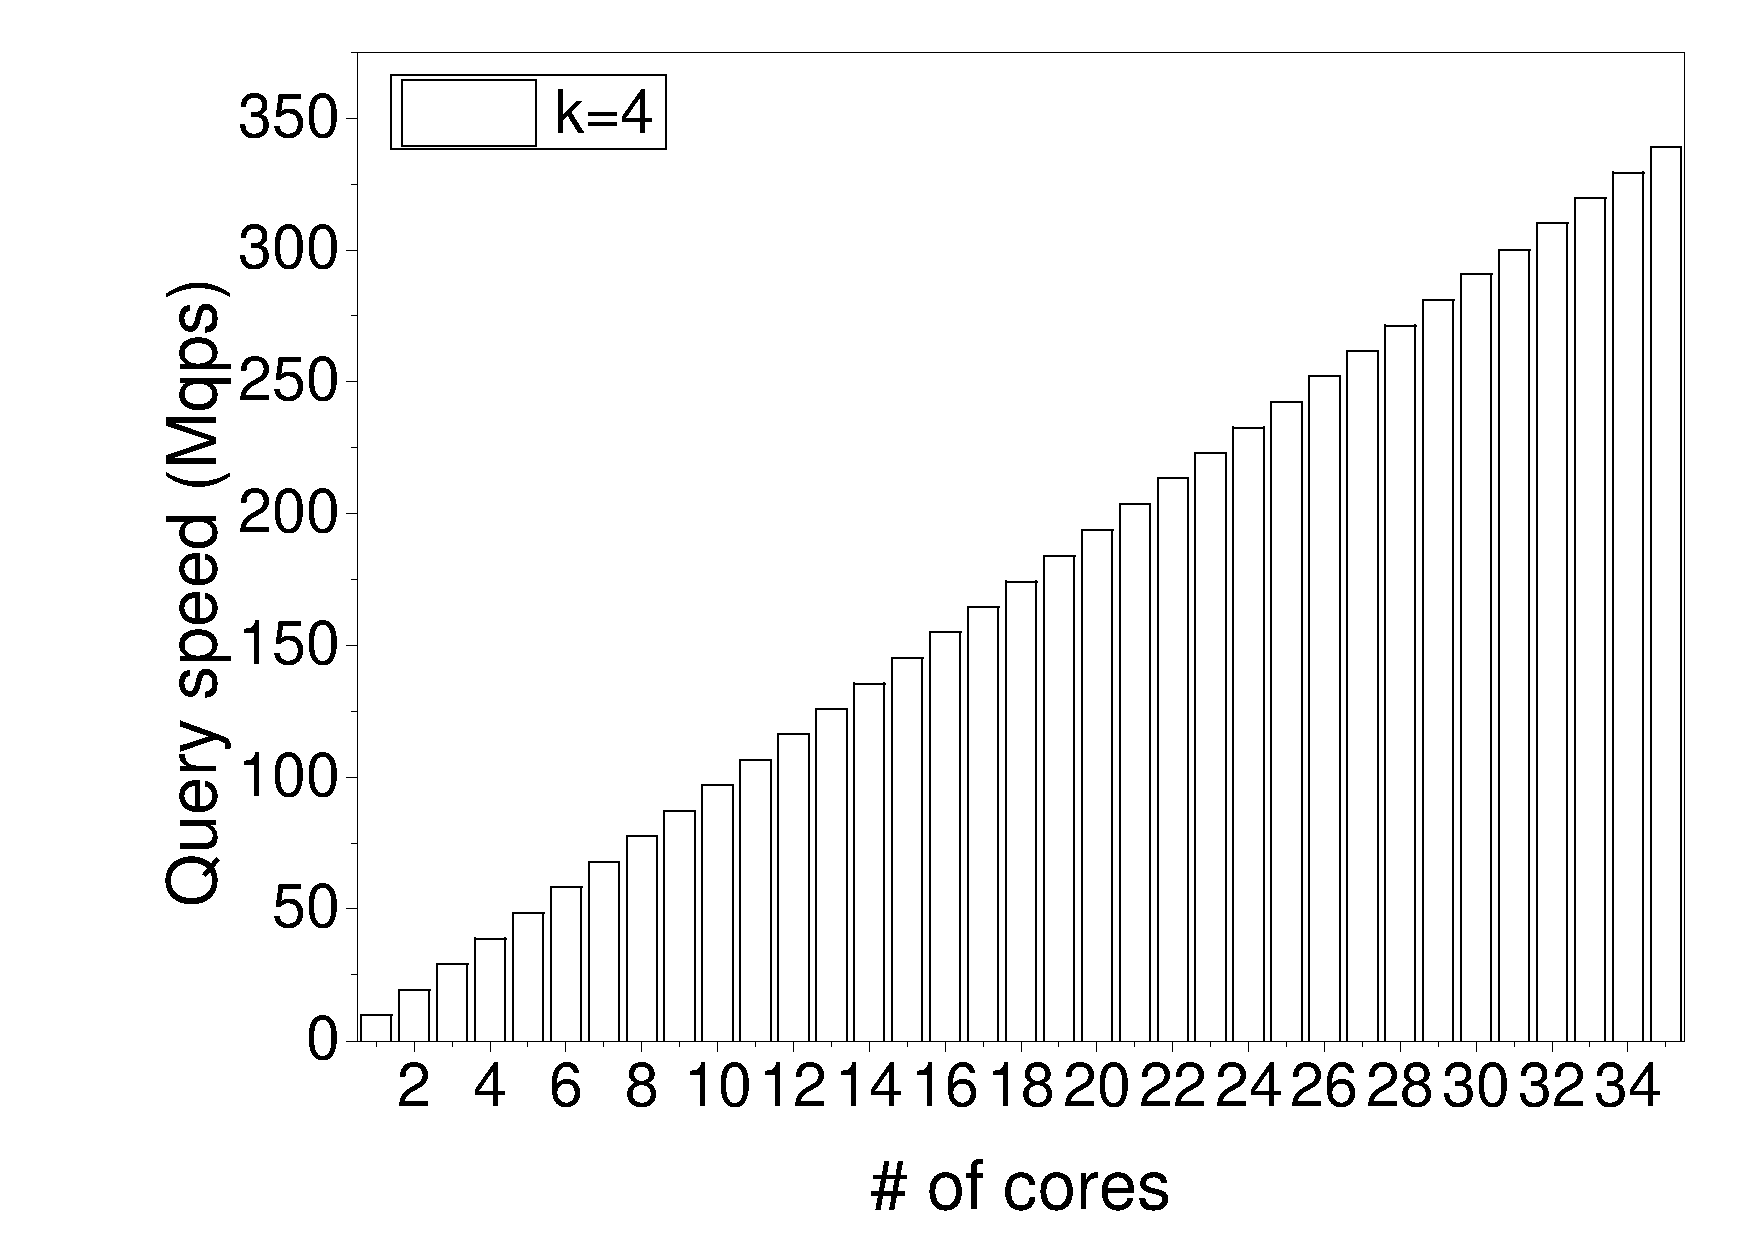
\includegraphics[width=6.2cm]{manyCoreTraffic1}}
 %		\centerline{(a) k=4}
 %	\end{minipage}
 %	\hfill
 %	\begin{minipage}{0.28\linewidth}
 %		\centerline{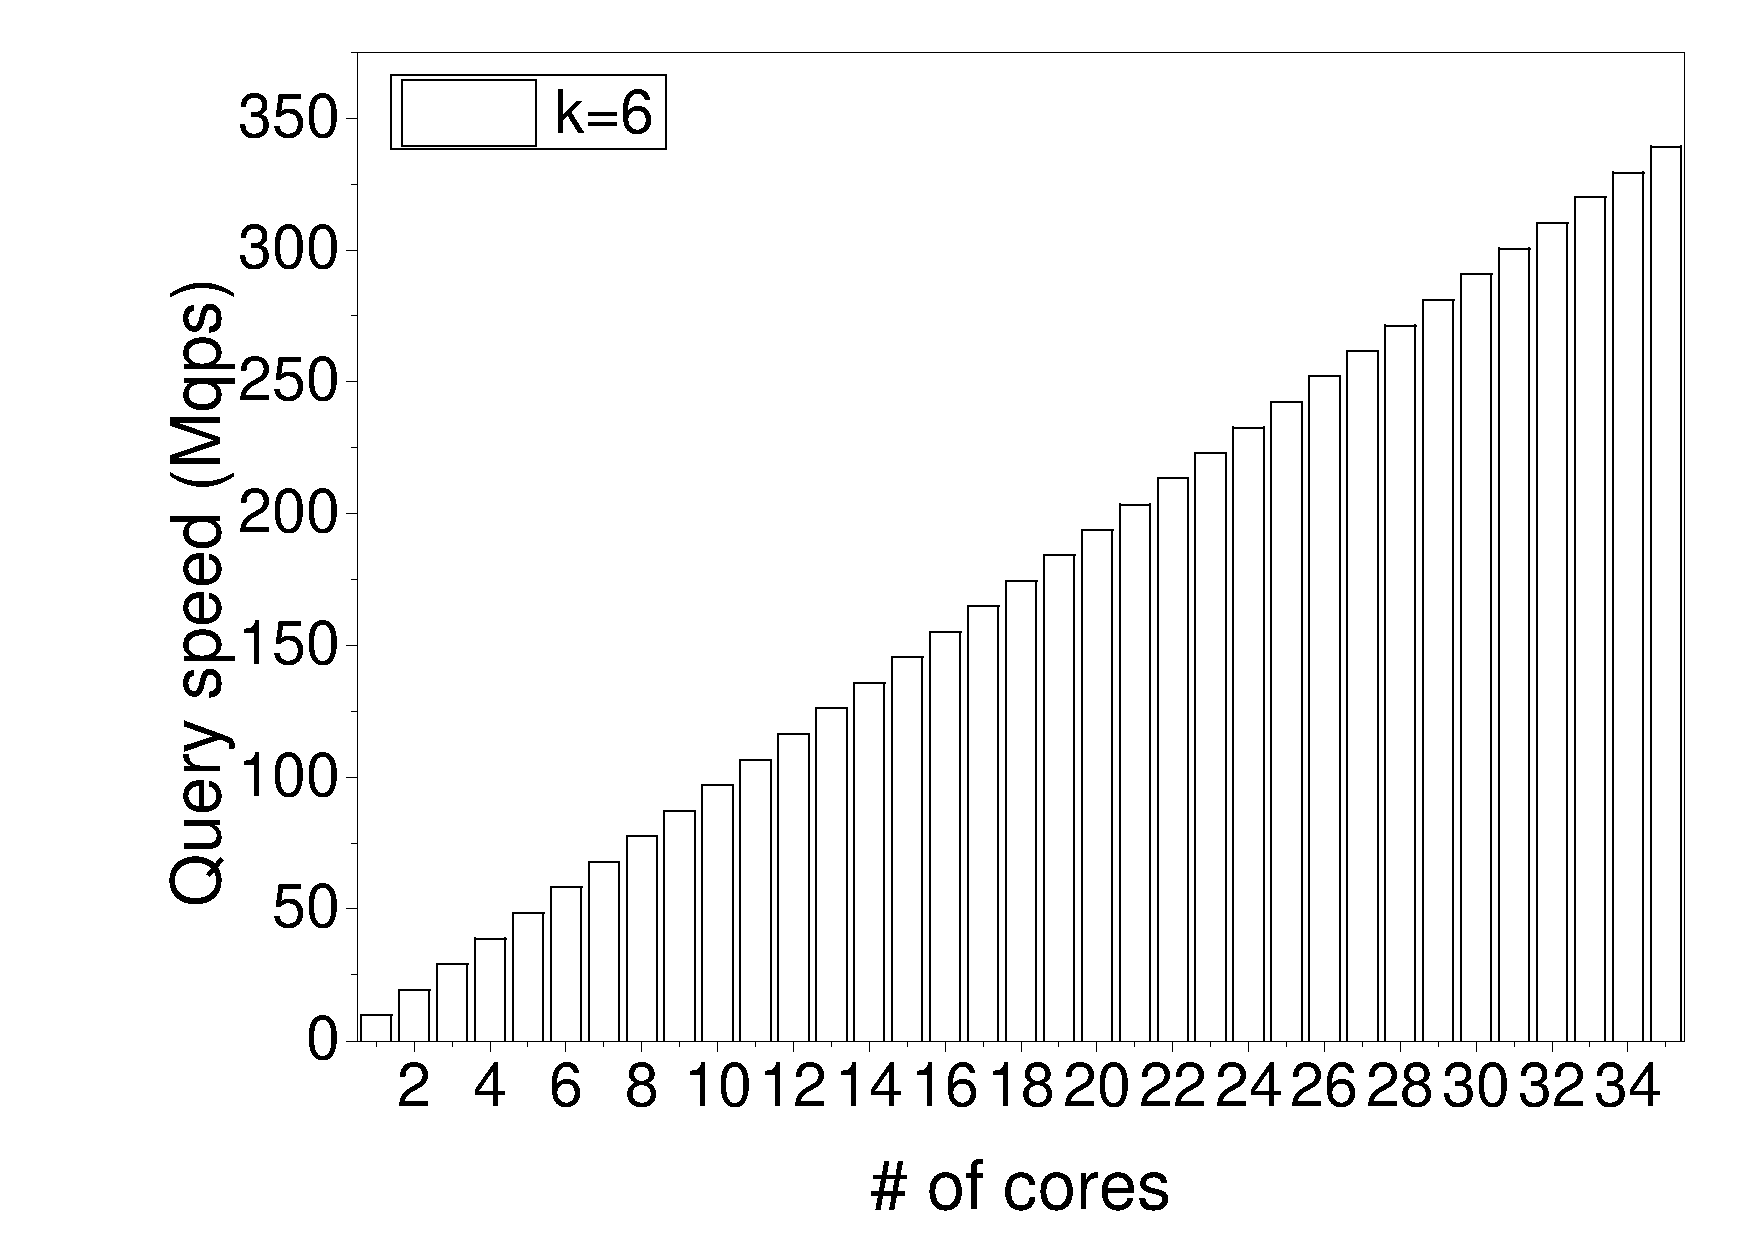
\includegraphics[width=5.8cm]{manyCoreTraffic2}}
 %		\centerline{(b) k=6}
 %	\end{minipage}
 %	\hfill
 %	\begin{minipage}{0.28\linewidth}
 %		\centerline{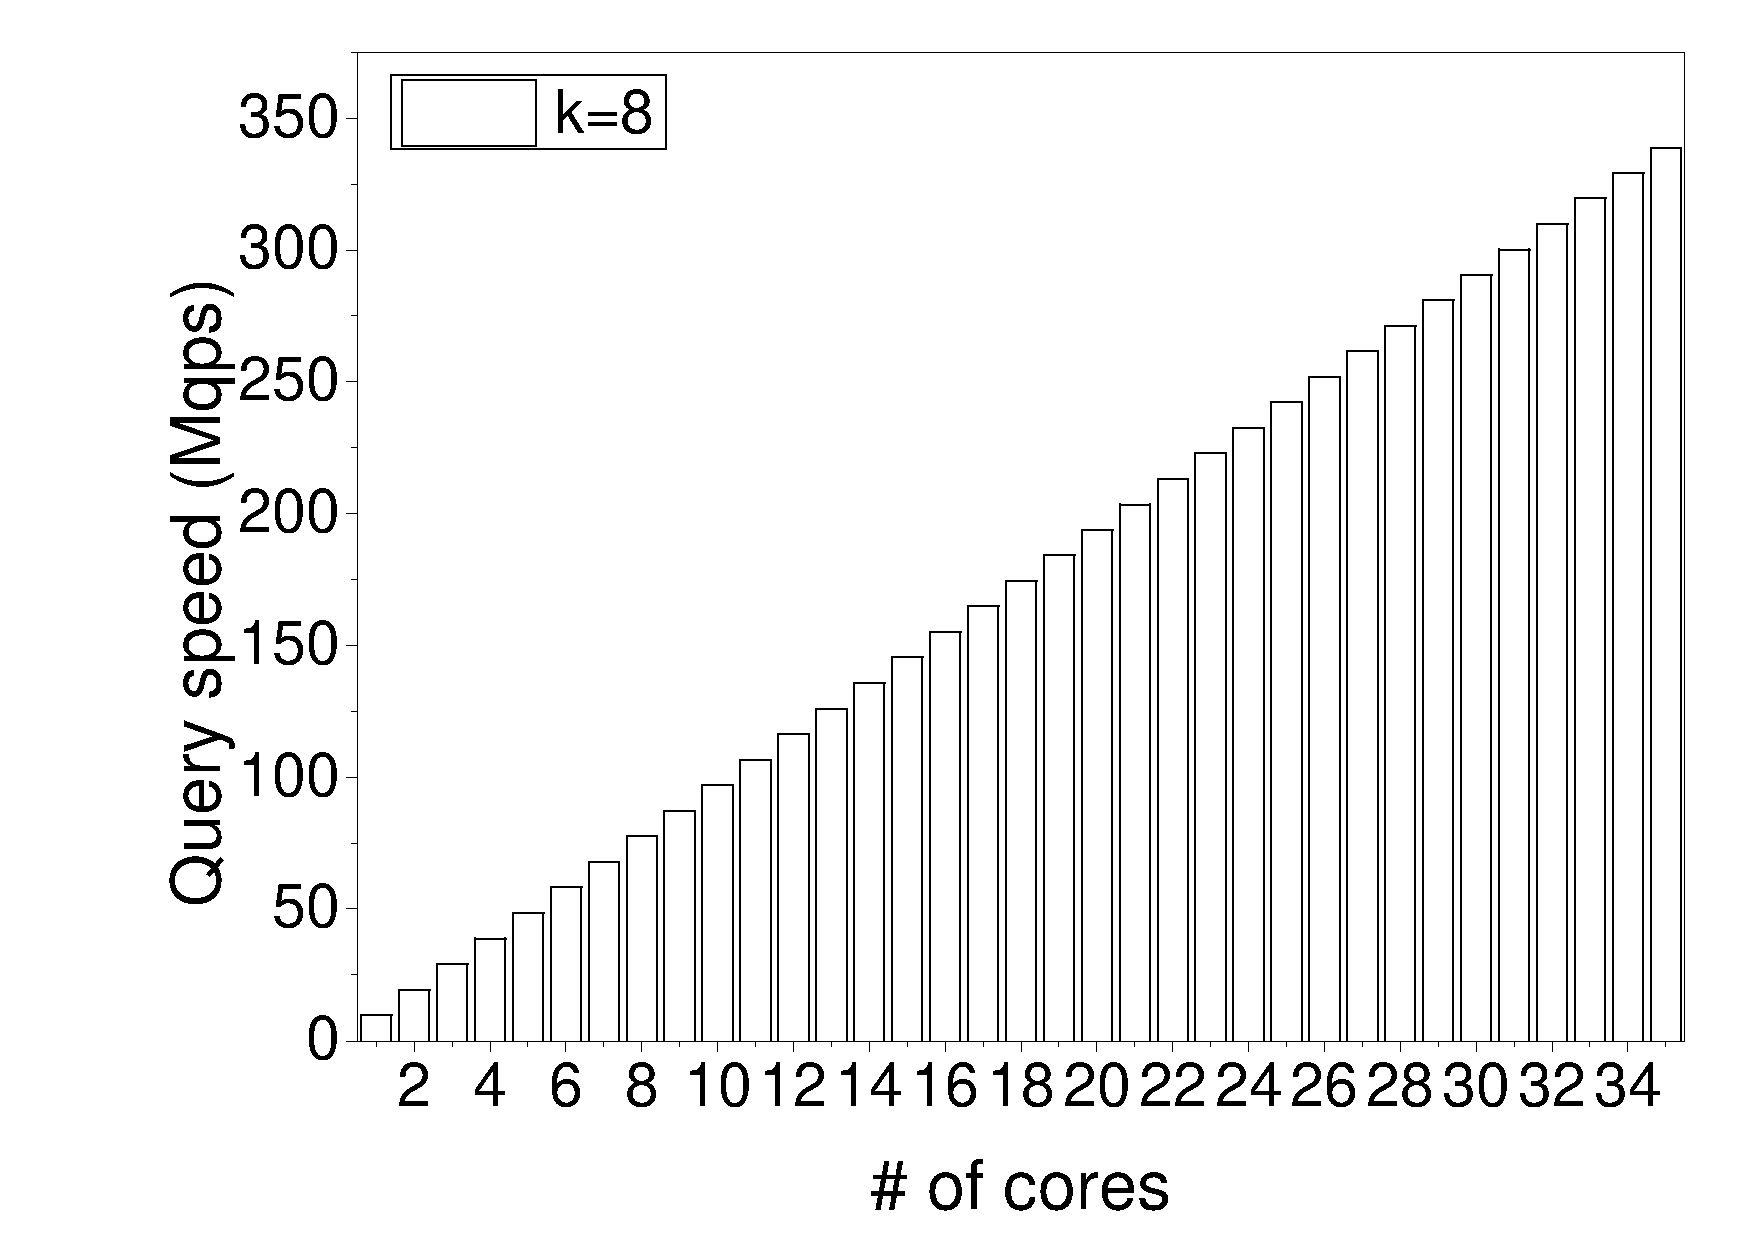
\includegraphics[width=5.8cm]{manyCoreTraffic3}}
 %		\centerline{(c) k=8}
 %	\end{minipage}
 %	\caption{Query speed VS. \# of cores.} \vspace{0in}
 %	\label{fig:manycore:QPS}
 %\end{figure*}

It can be seen from Figure \ref{fig:bestk} that the optimal $k$s are totally identical between the theoretical and practical results. For example, when $m=100,000$, $n=12,000$ and the best $k$ should be 5.78 obtained from our formula \ref{equ:mykform}. Since $k$ is an integer, we set $k=6$. In this experiment, when $k$ is 6, the FP probability is the lowest, which is 1.816\% in the 15 spots ranging from 2 to 16. The same logical also applied to other cases when $n$ is 8,000 and 10,000.

%\presub
%\subsection{Performance Test on CPU and Many-core Platform} \postsub

 %To better understand the SBF, we conduct the performance test of SBF on two platforms: CPU and Many-core.

 %\subsubsection{Performance on CPU}

 %We run the program on the same computer described above in the experimental setup section. We set up the SBF with the parameter $n=5000$, $k=4,6,8$ respectively and $m$ to be optimal according to the formula \ref{formulaM}. Then we query 100,000,000 elements in the 100M-traffic file. And for each 1,000,000 queries, we sum up the running time and calculate the query speed. The 100 spots are showed in Figure \ref{fig:PC:QPS}. The average query speed is $13.068Mqps$ (Million queries per second) when $k=4$, $12.496Mqps$ when $k=6$, and $12.326Mqps$ when $k=8$.




 %\subsubsection{Performance on Many-core Platform}

 %We also evaluated the query speed on the SBF versus the number of cores. We carry out experiments on the many-core platform Telera TLR4-03680. The many-core processor has 36 cores with a 256K L2 cache for each one. One L2 cache access needs 9 cycles.

 %In our implementation of the C++ program on many-core platform, we set one core to serve as the main thread and all other 35 cores to be the query threads. Also the main thread is in charge of dividing and distributing 35,000,000 elements (also from the beginning of the 100M traffic file) to 35 groups. Each group has 1,000,000 elements to be queried by one core and each core has its own SBF instance for querying. Of course, the SBF instances in the 35 cores are exactly the same with each other. We set up the SBF with the parameters $n=5000$, $k=4,6,8$ respectively and $m$ to be optimal according to the formula \ref{formulaM}.

 %Our experimental results are showed in Figure \ref{fig:manycore:QPS}. We can see that as the number of cores grows, the query speed increases linearly. Note that because one core is responsible for the main thread, which distributes the elements and collects the results from other cores, we only have the results of 35 cores. And the query speed can achieve $339Mqps$ when $k=4$ and 35 cores are running in parallel.








\presec
\newpage
%\vspace{-0.4in}
%\vspace{-0.07in}
\section{Correct Rate of Counting Bloom Filters}\postsec
\label{sec:cbfcr}
%\vspace{-0.03in}
The counting Bloom filter (CBF) \cite{cbf}, one widely used variant of standard Bloom filter, replaces each bit with one counter, supporting estimating the frequency of each element in a multiset. 
Specifically, given a multiset $\mathcal{S}$ of $n$ distinct elements with their corresponding frequencies, we create a counter array $A$ of length $m$ as follows. 
First, we initialize each counter of $A$ to 0, then for each element $x \in \mathcal{S}$, we use $k$ hash functions to compute $k$ hash values: $h_1(x), h_2(x),..., h_{k}(x)$ where each hash value is in the range $[1, m]$.
%
Second, for each $1 \leqslant i \leqslant k$, we let $A[h_i(x)]=A[h_i(x)] +1$.
%
Let $f_x$ be the frequency of element $x$ in multiset $\mathcal{S}$. 
% and its frequency $f_x$
Therefore, the step of $A[h_i(x)]=A[h_i(x)] +1~\text{for each}~1 \leqslant i \leqslant k$ will occur $f_x$ times. 
%
The resulting counter array $A$ is called the CBF for multiset $\mathcal{S}$.
%
To query the frequency of an element $y$ in multiset $\mathcal{S}$, we first use the same $k$ hash functions to compute $k$ hash values: $h_1(y), h_2(y),..., h_{k}(y)$.
%
Second, we report the minimum value of the $k$ counters: $A[h_1(x)], A[h_2(x)], ..., A[h_k(x)]$ as the estimated frequency of this element. 
%Second, we check whether the corresponding $k$ bits in $A$ are all $1s$ (\ie, whether $A[h_1(y)] \wedge A[h_2(y)] \wedge \cdots, A[h_{k}(y)]=1$ holds); if yes, then $y \in S$ may probably hold and we can further check whether $y \in S$; if no, then $y \in S$ definitely does not hold.
%
Obviously, the estimated frequency reported by the CBF is always  larger than or equal to the real frequency for any element in multiset $\mathcal{S}$. 
The case that the estimated frequency from the CBF is equal to the real frequency for one element is called the correct case. 
The probability of such case happening is called the correct rate of the CBF ($\mathcal{C}_r$). 
%%
%The FP probability $f$ can be calculated from $n$, $k$, and $m$.


The calculation of the correct rate of CBFs can benefit from our derivation of the false positive probability of standard Bloom filter.
In querying an element $x$, the correct case happens when there exists at least one hashed counter (among $A[h_1(x)], A[h_2(x)], ..., A[h_k(x)]$) that is not hashed by any elements in multiset $\mathcal{S} \setminus \{x \cdot f_x\}$. 
The contrapositive is that the correct case does not happen when all the $k$ hashed counters are also hashed by some elements in multiset $\mathcal{S} \setminus \{x \cdot f_x\}$. 
%the false positive happens when the Bloom filter reports that $y \in \mathcal{S}$ (\ie, $A[h_i(x)]=1$ holds for each $1 \leqslant i \leqslant k$), but actually $x \notin \mathcal{S}$.
Consider an arbitrary counter $A[b]$ in $A$.
%
For any distinct element in $\mathcal{S} \setminus \{x \cdot f_x\}$ and any hash function $h_i$ ($1 \leqslant i \leqslant k$), the probability that this element is not hashed to counter $A[b]$ by $h_i$ is $1-1/m$.
%
As $\mathcal{S} \setminus \{x \cdot f_x\}$ has $n-1$ distinct elements and each distinct element is hashed $k$ times, the probability that $A[b]$ is not hashed by any element in multiset $\mathcal{S} \setminus \{x \cdot f_x\}$ is $p_c$:
%
\begin{equation}
p_c=\left(1-\dfrac{1}{m}\right)^{k(n-1)}
\label{pform_c}
\end{equation}
%
Thus, the probability that $A[b]$ is hashed by some elements in multiset $\mathcal{S} \setminus \{x \cdot f_x\}$ is $1-(1-1/m)^{k(n-1)}$. 
The probability that all the $k$ hashed counters are also hashed by some elements in multiset $\mathcal{S} \setminus \{x \cdot f_x\}$ is answered by $f_{true}$ with element number of $n-1$. 
We denote $f_{true}|_{n-1}$ as $f_{true}$ with element number of $n-1$, and get: 
\begin{equation}
1 - \mathcal{C}_r = f_{true}|_{n-1} \Rightarrow \mathcal{C}_r = 1 - f_{true}|_{n-1}
\end{equation}
Applying Eq. \ref{bounds}, we can get the upper and lower bounds of the $\mathcal{C}_r$ of CBFs: 
\begin{equation}
{\small
\begin{aligned}
\label{cbfbounds}
1 - \left( 1- \left( 1-\dfrac{k}{m} \right)^{n-1} \right) ^k < \mathcal{C}_r < 1 - \left( 1- \left( 1-\dfrac{1}{m} \right)^{(n-1)k} \right) ^k
\end{aligned}
}
\end{equation}


\presec
\section{Experimental Results} \postsec
\label{sec:evaluation}
%The goal of this section is to validate the accuracy and correctness of our proposed bound and formula.
In this section, we first validate our proposed formula of optimal $k$ (Eq. \ref{equ:mykform}).
Second, we compare our proposed upper bound of the FP probability of BFs (Eq. \ref{bounds}) with Bose's upper bound (Eq. \ref{fBound}). 
Third, we validate our proposed upper and lower bounds of the correct rate of CBFs (Eq. \ref{cbfbounds}). 

\presub
\subsection{Experimental Setup}\postsub
\label{setup}

\noindent\textbf{Datasets: }
%\para{}
We use the anonymized IP trace collected in 2016 from CAIDA \cite{caida}.
Each flow is identified by its source IP address (sip) and destination IP address (dip). 
For BF, each distinct sip-dip pair from this trace functions as an element in the aforementioned set. 
We use (part of) the first 100M distinct sip-dip pairs to construct BFs, and query the next 300M distinct sip-dip pairs to get the empirical FP probabilities of these BFs. 
For CBF, each distinct sip-dip pair and its occurrence number from this trace function as a distinct element and the corresponding frequency in the aforementioned multiset, respectively. 
We use (part of) the first 100M distinct sip-dip pairs and their occurrence numbers in the current trace to construct CBFs, and query their frequencies to get the empirical correct rates of these CBFs. 

\noindent\textbf{Implementation: }
We have implemented the standard Bloom filter in C\texttt{++}.
We use the Bob Hash (obtained from the open source website \cite{bobhash}) with different initial seeds to implement the hash functions in BFs as recommended by literature \cite{hashformeasure}. 
All the implementation source code is made publicly available anonymously at GitHub \cite{opensource}.

%\noindent\textbf{Computation Platform: }
%We performed all the experiments on a machine with 12-core CPUs (24 threads, Intel Xeon CPU E5-2620 @2 GHz) and 62 GB total DRAM memory.
%Each CPU core has three levels of cache memory: two 32KB L1 caches (one is a data cache and the other is an instruction cache) for each core, one 256KB L2 cache for each core, and one 15MB L3 cache shared by all cores.

\subsection{Optimal $k$ Formula Validation}

\subsubsection{Optimal $k$ vs. $n$}
Figure \ref{opt_k_n} plots the empirically and theoretically optimal $k$ with different $n$ increasing from 10M to 100M with a step of 10M for $m = 500$M. 
\textit{Our results show that the optimal $k$ calculated from our new formula follows the empirically optimal $k$ very well, regardless of the values of $n$.} 
We observe that the optimal $k$ calculated from our new formula is very close to the one calculated from the formula obtained by Bloom. 
The reason is that the above two formulas about the optimal $k$ have the same asymptotic form when $m$ is large enough (see Section \ref{optk}). 


\begin{figure}[t]
	\centering
	\prefig
	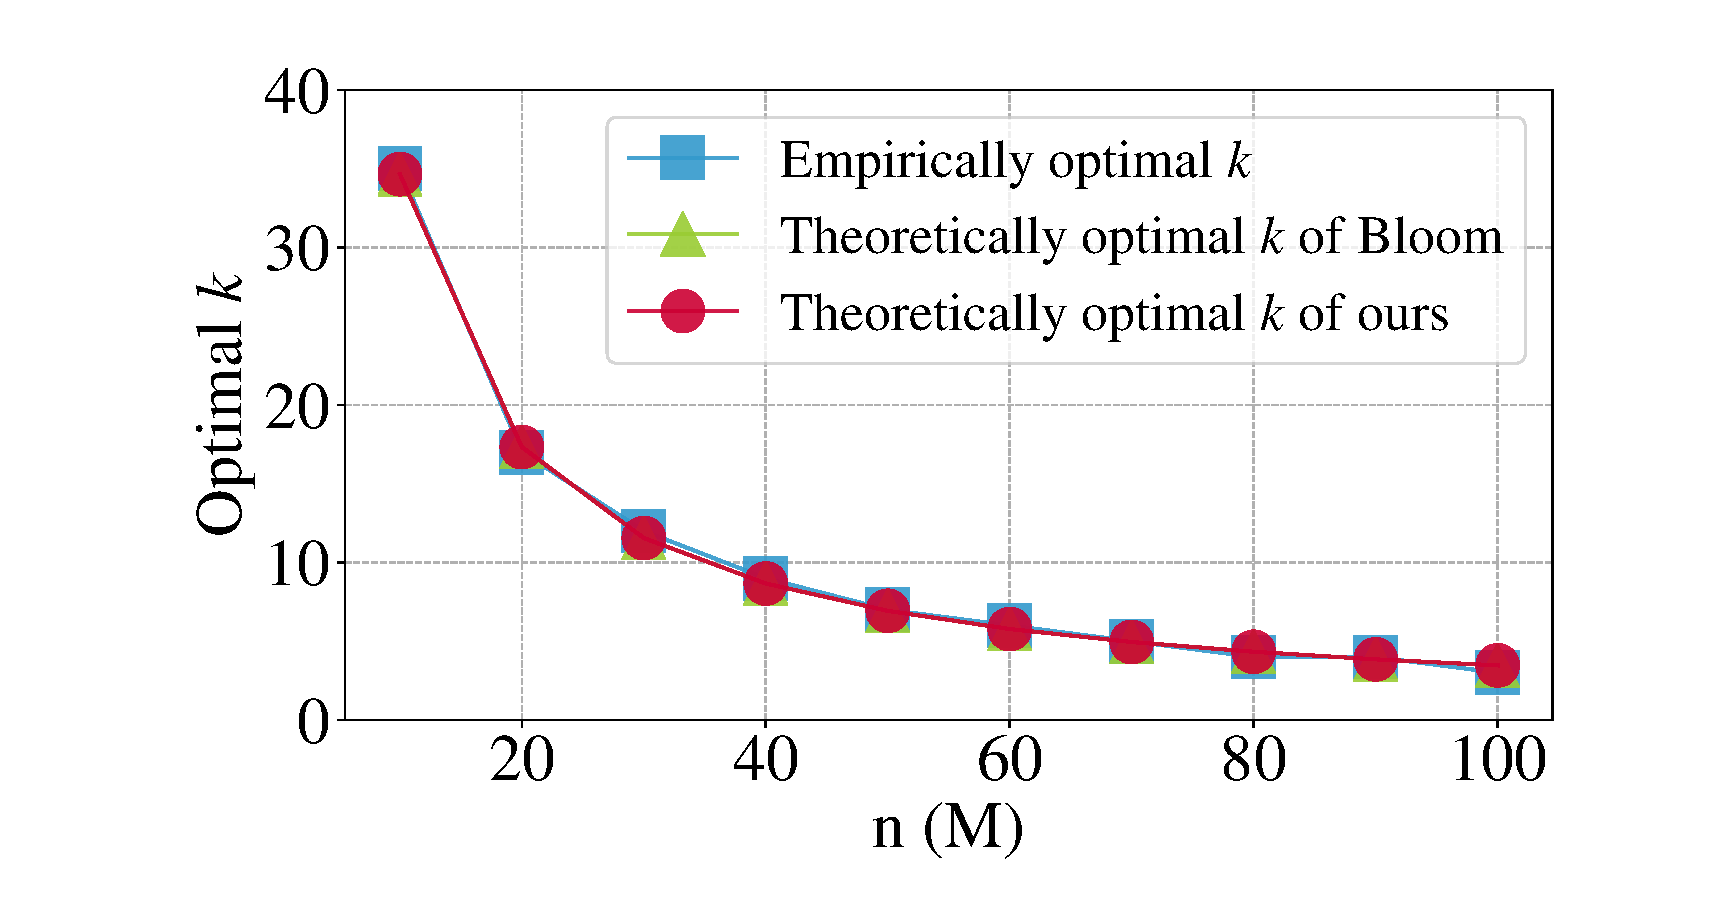
\includegraphics[width=0.288\textwidth]{opt_k_n}
	\postfig
	\precaption\adjustfigs
	\caption{Optimal $k$ vs. $n$ for $m = 500$M.}
	\postcaption
	\label{opt_k_n}
	\vspace{0.05in}
\end{figure}


\subsubsection{Optimal $k$ vs. $m$}

Figure \ref{opt_k_m} plots the empirically and theoretically optimal $k$ with different $m$ increasing from 100M to 1000M with a step of 100M for $n = 50$M. 
\textit{Our results show that the optimal $k$ calculated from our new formula follows the empirically optimal $k$ very well, regardless of the values of $m$.} 
We observe that the optimal $k$ calculated from our new formula is very close to the one calculated from the formula obtained by Bloom, especially when $m$ becomes larger. 
%The reason is that the above two formulas about the optimal $k$ have the same asymptotic form when $m$ is large enough (see Section \ref{optk}). 

\begin{figure}[t]
	\centering
	\prefig
	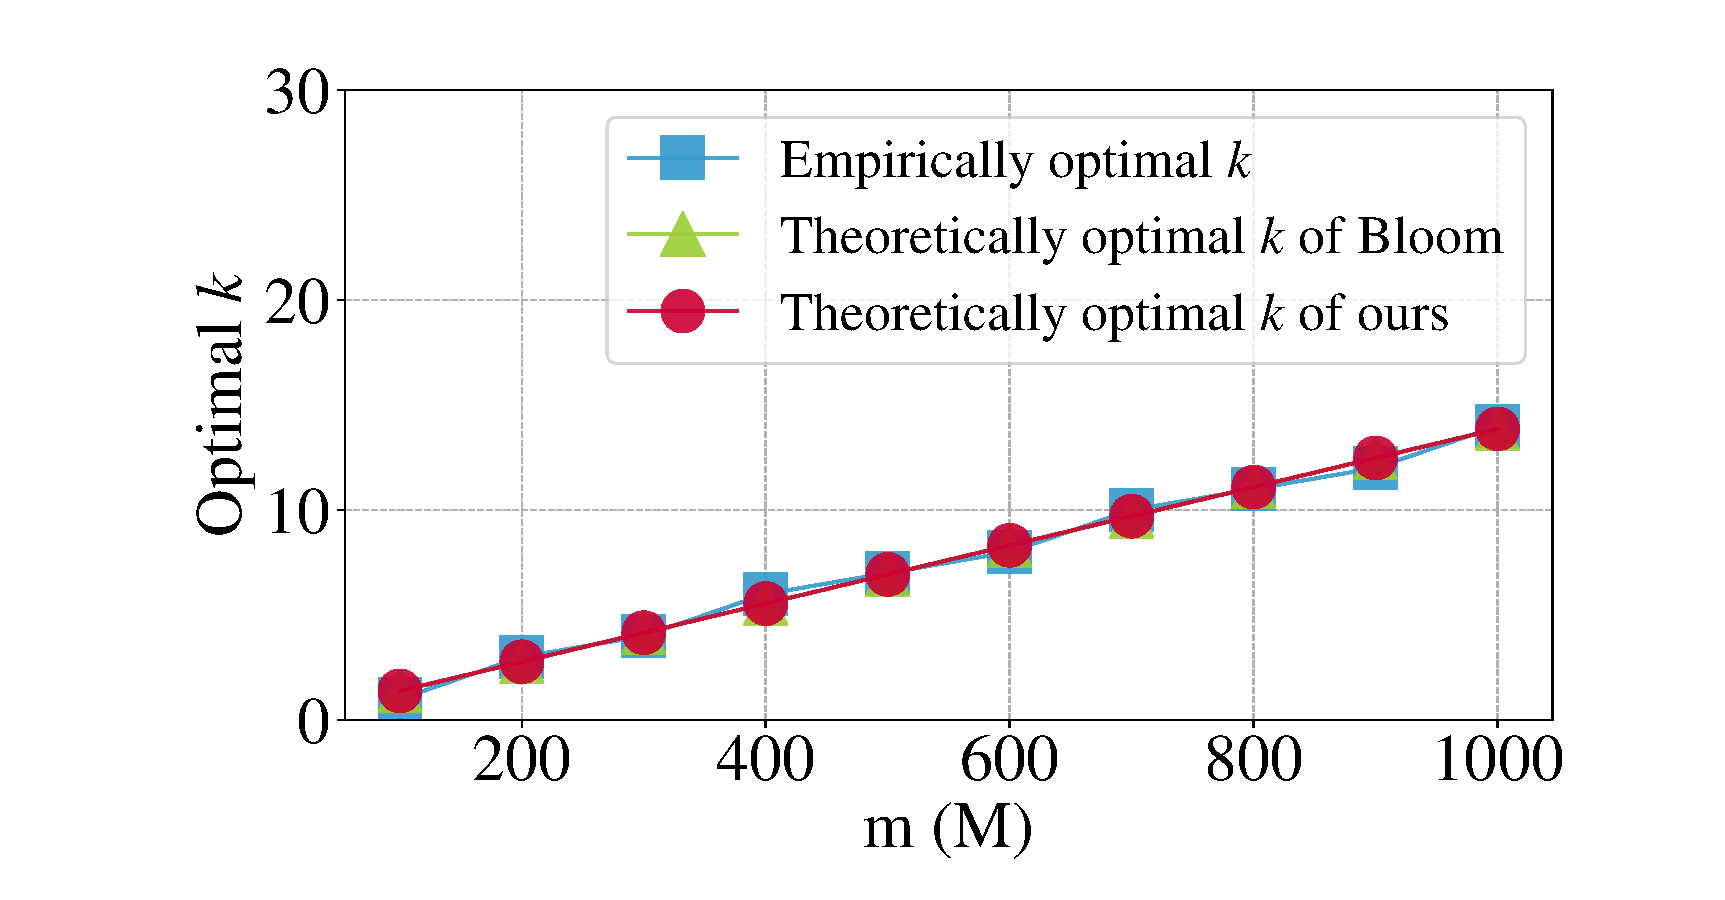
\includegraphics[width=0.288\textwidth]{opt_k_m}
	\postfig \precaption
	\adjustfigs
	\caption{Optimal $k$ vs. $m$ for $n = 50$M.}
	\label{opt_k_m}
	\postcaption
\end{figure}



%\vspace{-0.1in}
\subsection{Upper Bound Comparison}


\begin{figure*}[t!]
	\vspace{0.1in}
	\centering
	%
	\begin{minipage}[t]{0.32\textwidth}{
			\prefig
			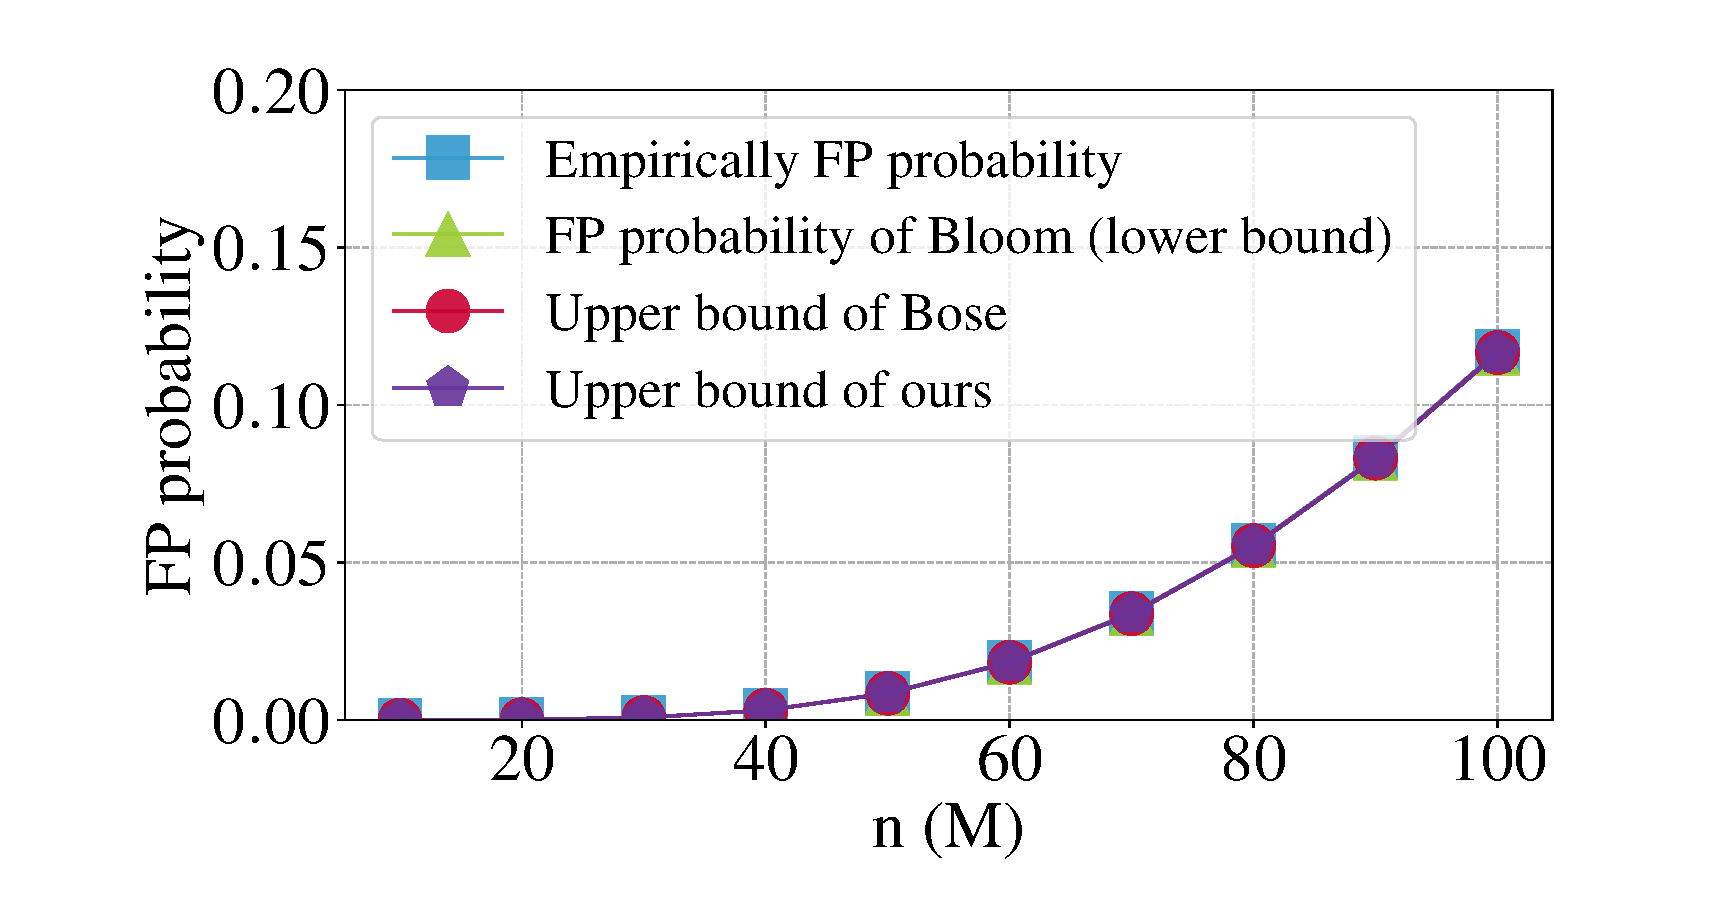
\includegraphics[width=0.90\textwidth, height=1.125in]{upbound_n}}
		\postfig\precaption\adjustfigs
%		\vspace{-0.05in}
		\caption{FP probability vs. $n$ for $m = 500$M and $k = 6$.}
		\label{upbound_n}\postcaption
	\end{minipage}
	%
	\begin{minipage}[t]{0.32\textwidth}{
			\prefig
			\vspace{0.02in}
			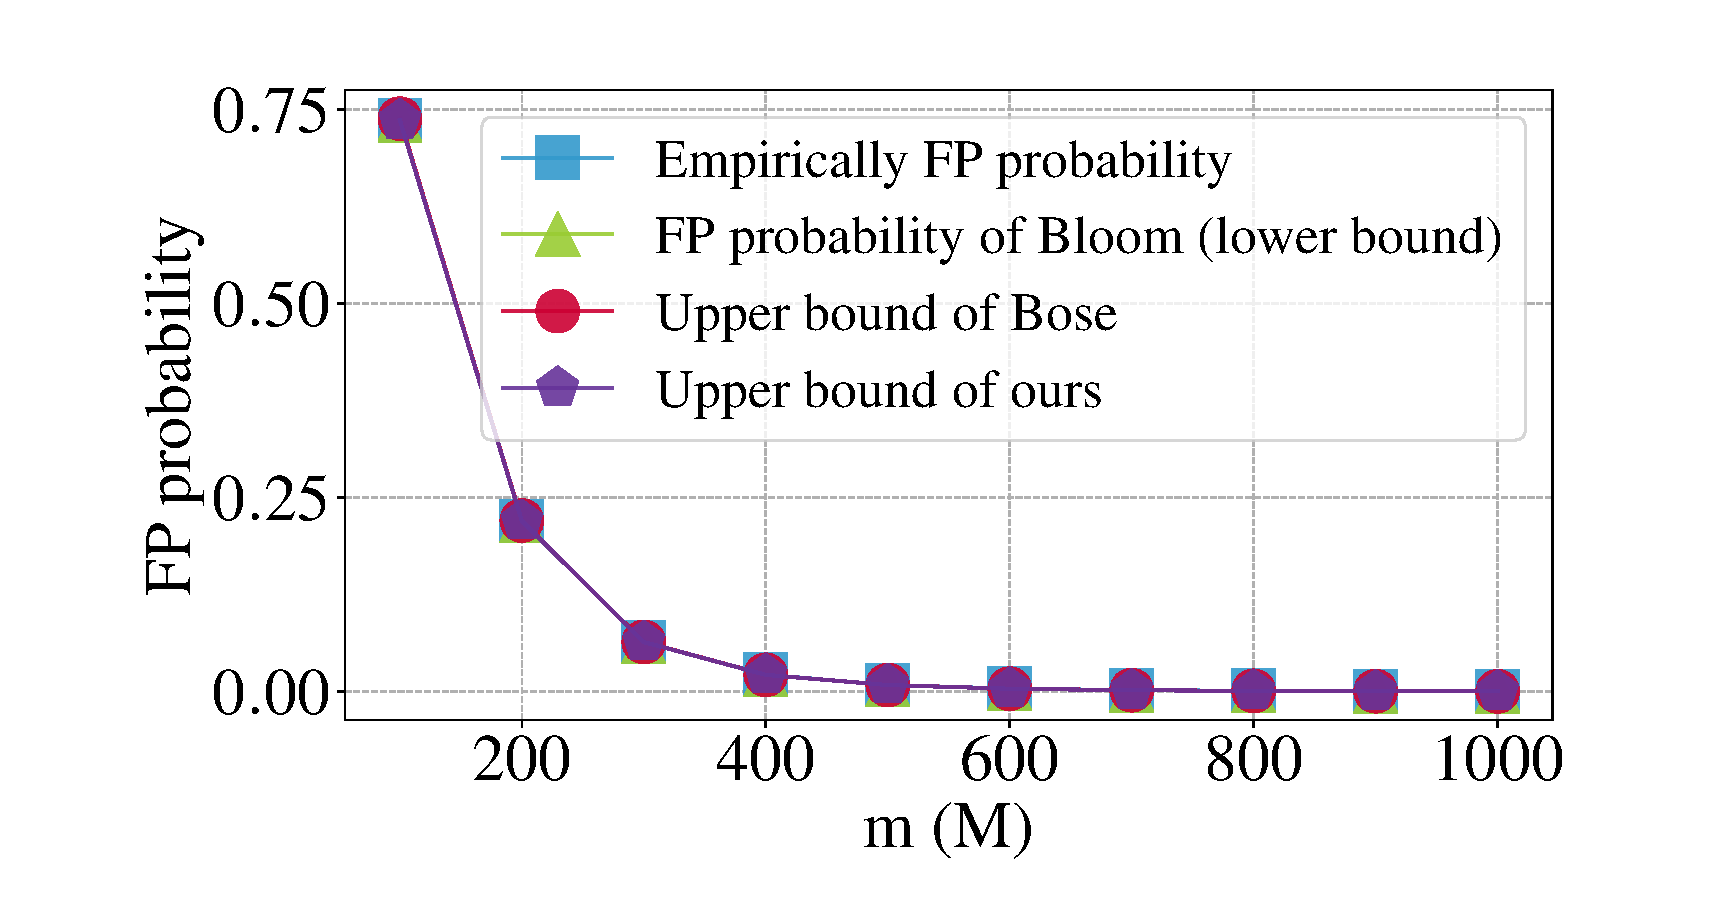
\includegraphics[width=0.90\textwidth, height=1.125in]{upbound_m}}
			\vspace{-0.02in}
		\postfig\precaption\adjustfigs
%		\vspace{-0.05in}
		\caption{FP probability vs. $m$ for $n = 50$M and $k = 6$.}
		\label{upbound_m}\postcaption
	\end{minipage}
	%
	\begin{minipage}[t]{0.32\textwidth}{
			\prefig
			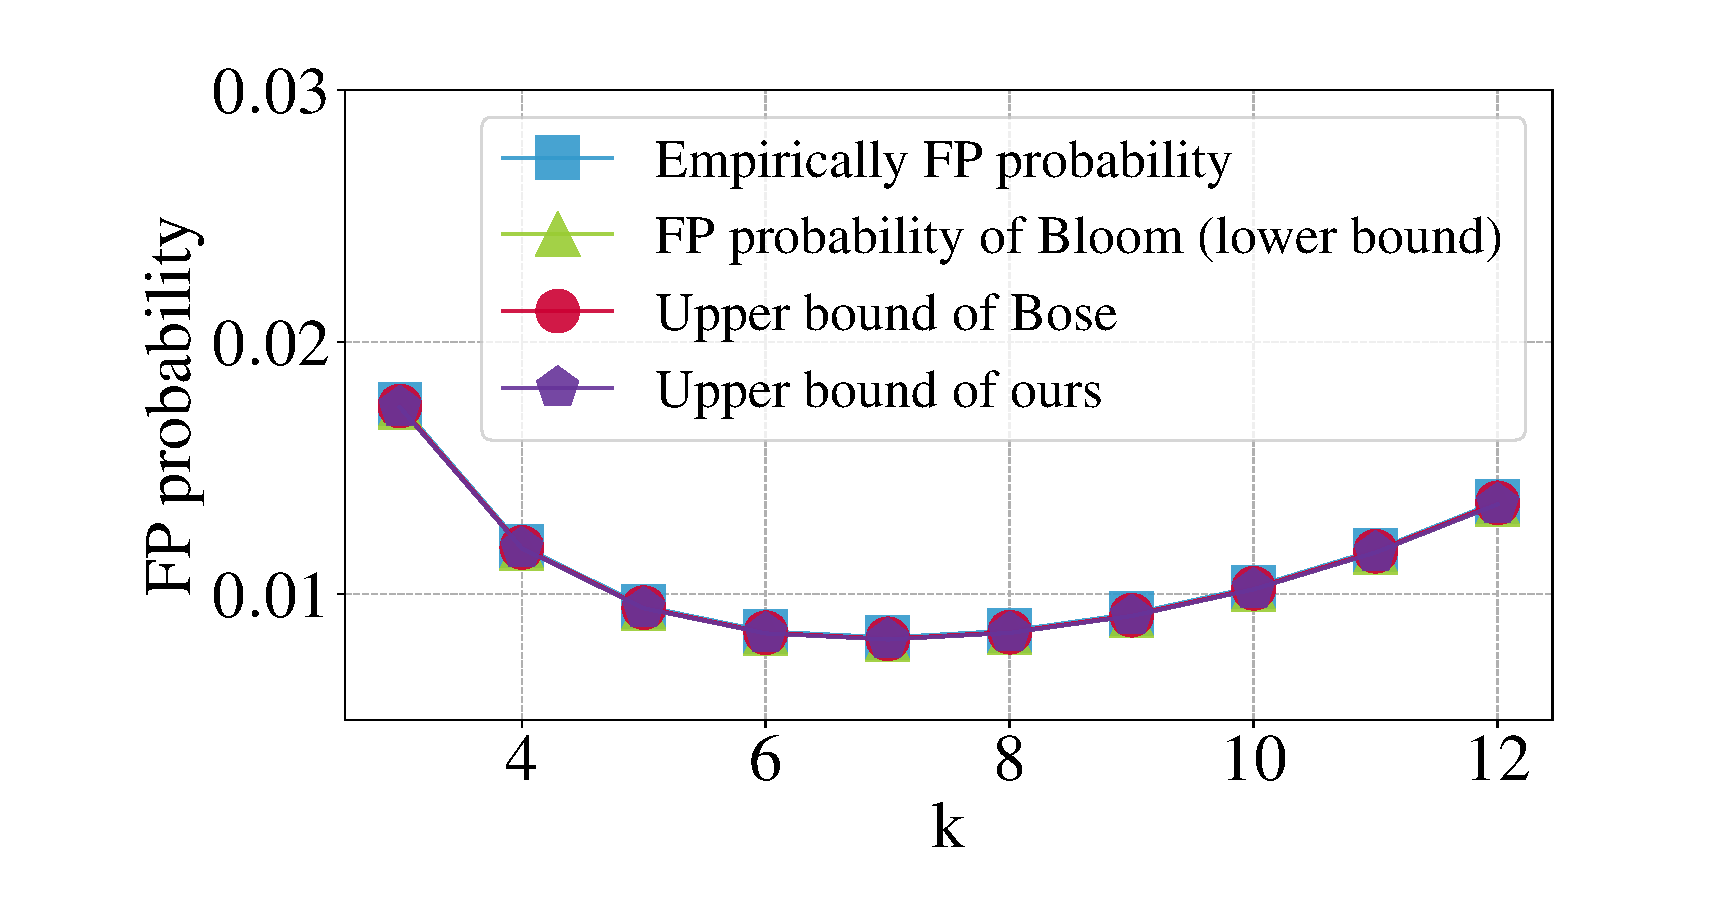
\includegraphics[width=0.90\textwidth, height=1.125in]{upbound_k}}
		\postfig\precaption\adjustfigs
%		\vspace{-0.05in}
		\caption{FP probability vs. $k$ for $n = 50$M and $m = 500$M.}
		\label{upbound_k}\postcaption
	\end{minipage}
	%
%	\vspace{-0.02in}
\end{figure*}

\begin{figure*}[t!]
	\vspace{0.1in}
	\centering
	%
	\begin{minipage}[t]{0.32\textwidth}{
			\prefig
			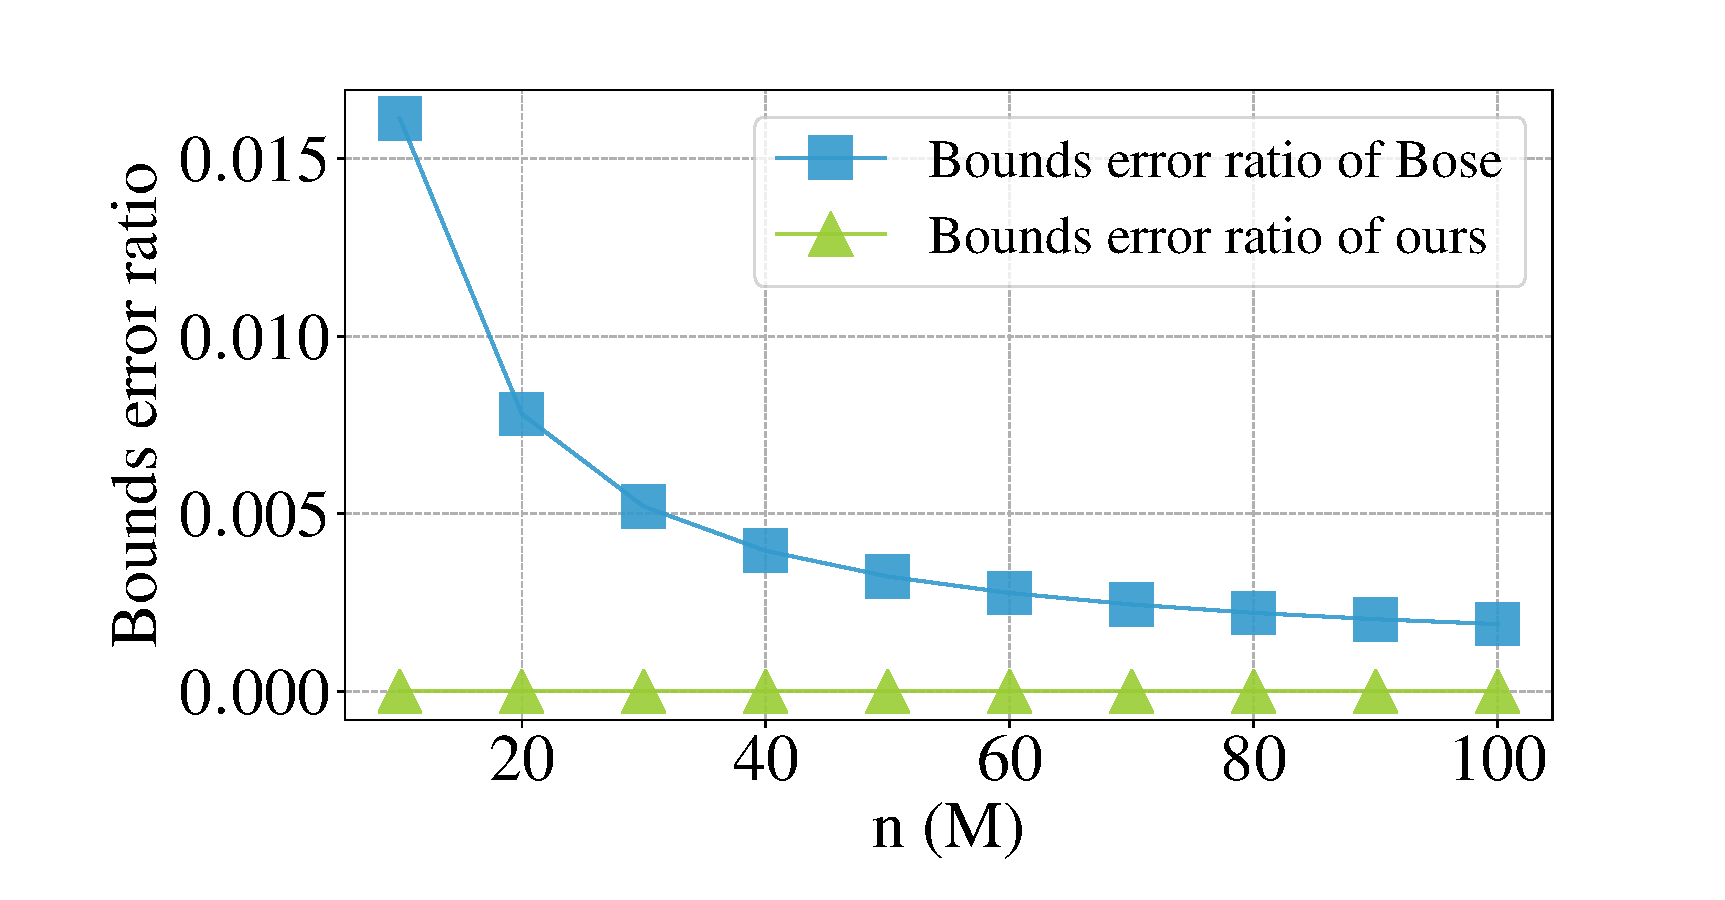
\includegraphics[width=0.90\textwidth, height=1.125in]{upbound_error_ratio_n}}
		\postfig\precaption\adjustfigs
%		\vspace{-0.05in}
		\caption{Bounds error ratio vs. $n$ for $m = 500$M and $k = 6$.}
		\label{upbound_error_ratio_n}\postcaption
	\end{minipage}
	%
	\begin{minipage}[t]{0.32\textwidth}{
			\prefig
			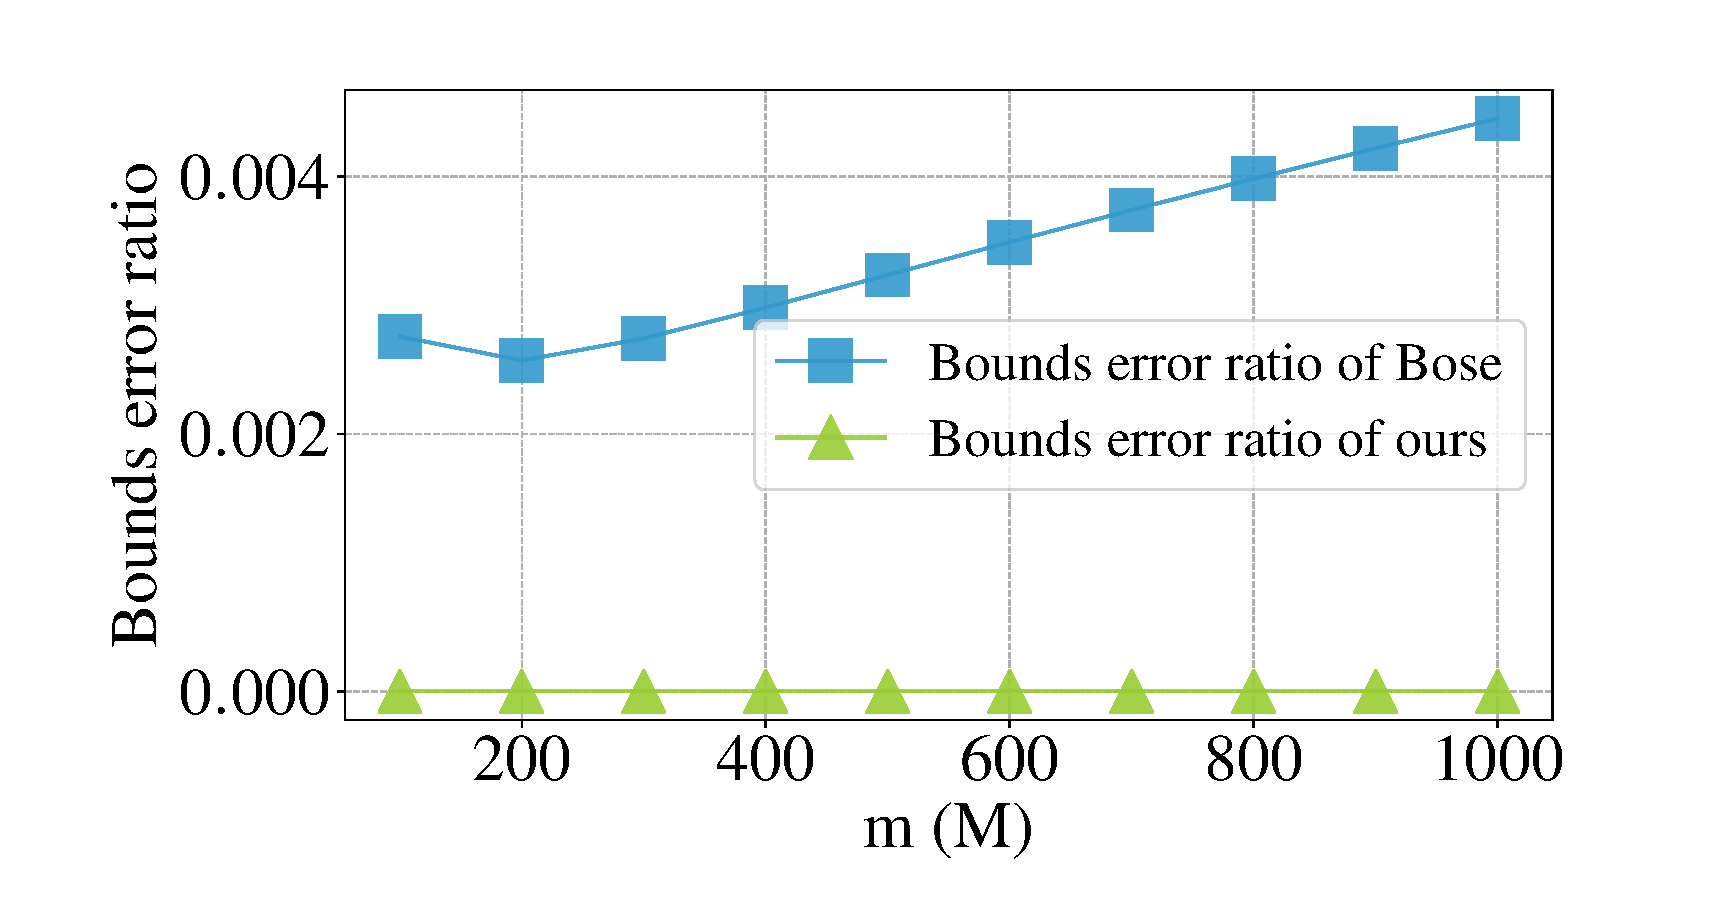
\includegraphics[width=0.90\textwidth, height=1.125in]{upbound_error_ratio_m}}
		\postfig\precaption\adjustfigs
%		\vspace{-0.05in}
		\caption{Bounds error ratio vs. $m$ for $n = 50$M and $k = 6$.}
		\label{upbound_error_ratio_m}\postcaption
	\end{minipage}
	%
	\begin{minipage}[t]{0.32\textwidth}{
			\prefig
			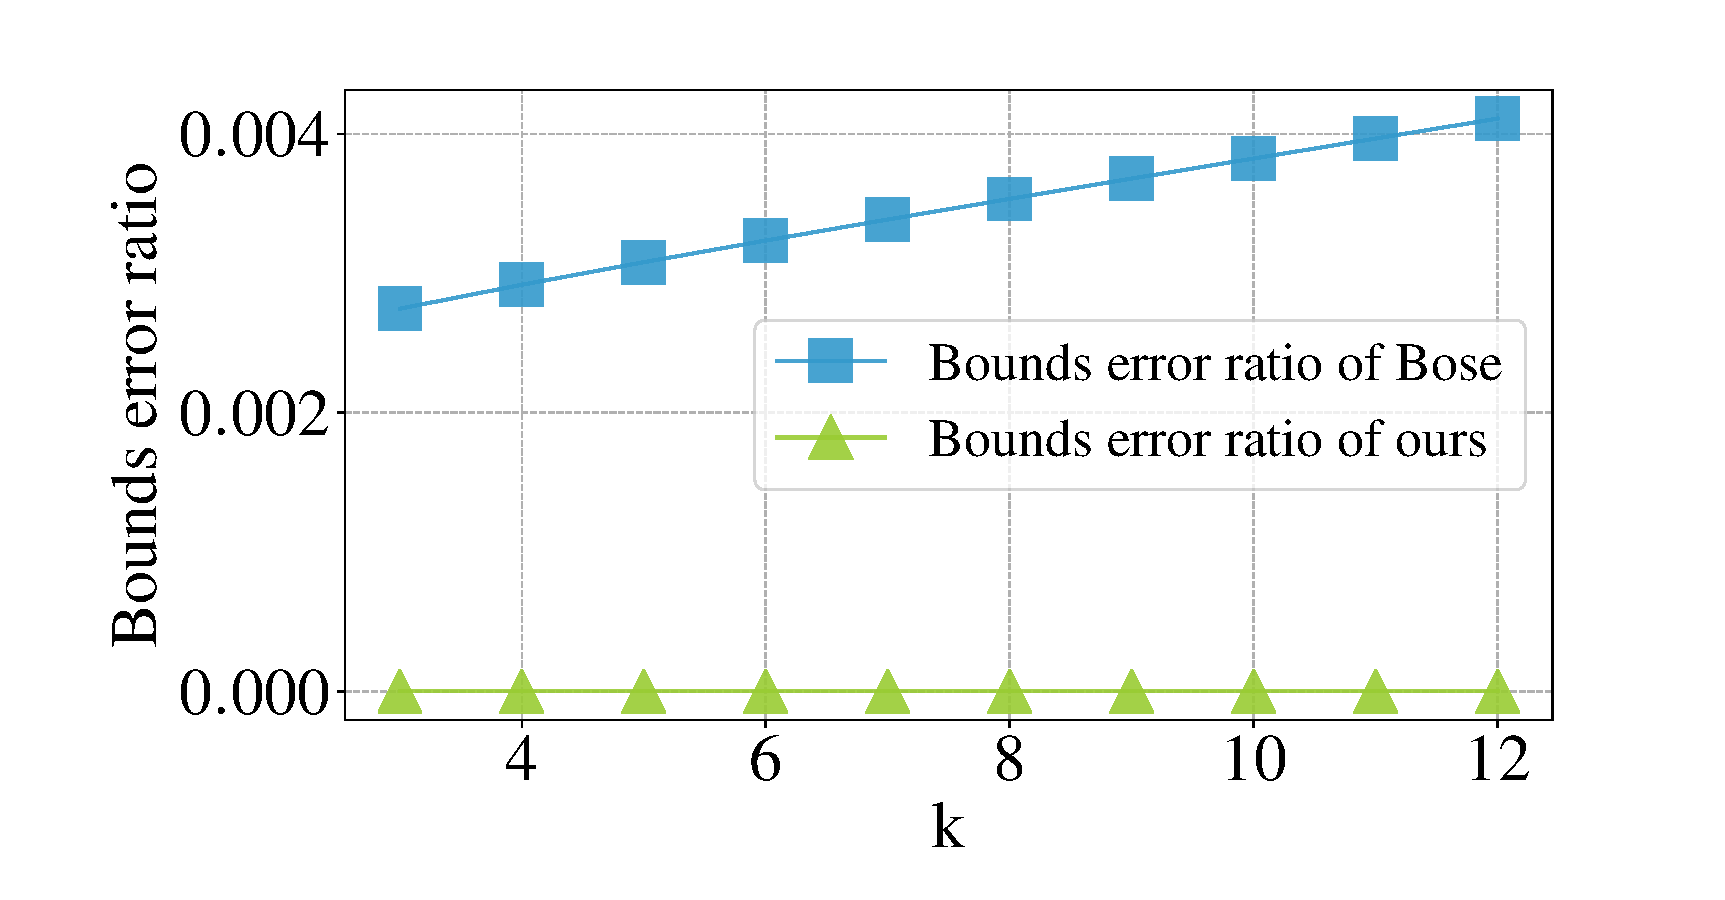
\includegraphics[width=0.90\textwidth, height=1.125in]{upbound_error_ratio_k}}
		\postfig\precaption\adjustfigs
%		\vspace{-0.05in}
		\caption{Bounds error ratio vs. $k$ for $n = 50$M and $m = 500$M.}
		\label{upbound_error_ratio_k}\postcaption
	\end{minipage}
	%
%	\vspace{-0.02in}
\end{figure*}

\begin{figure*}[t!]
	\vspace{0.1in}
	\centering
	%
	\begin{minipage}[t]{0.32\textwidth}{
			\prefig
			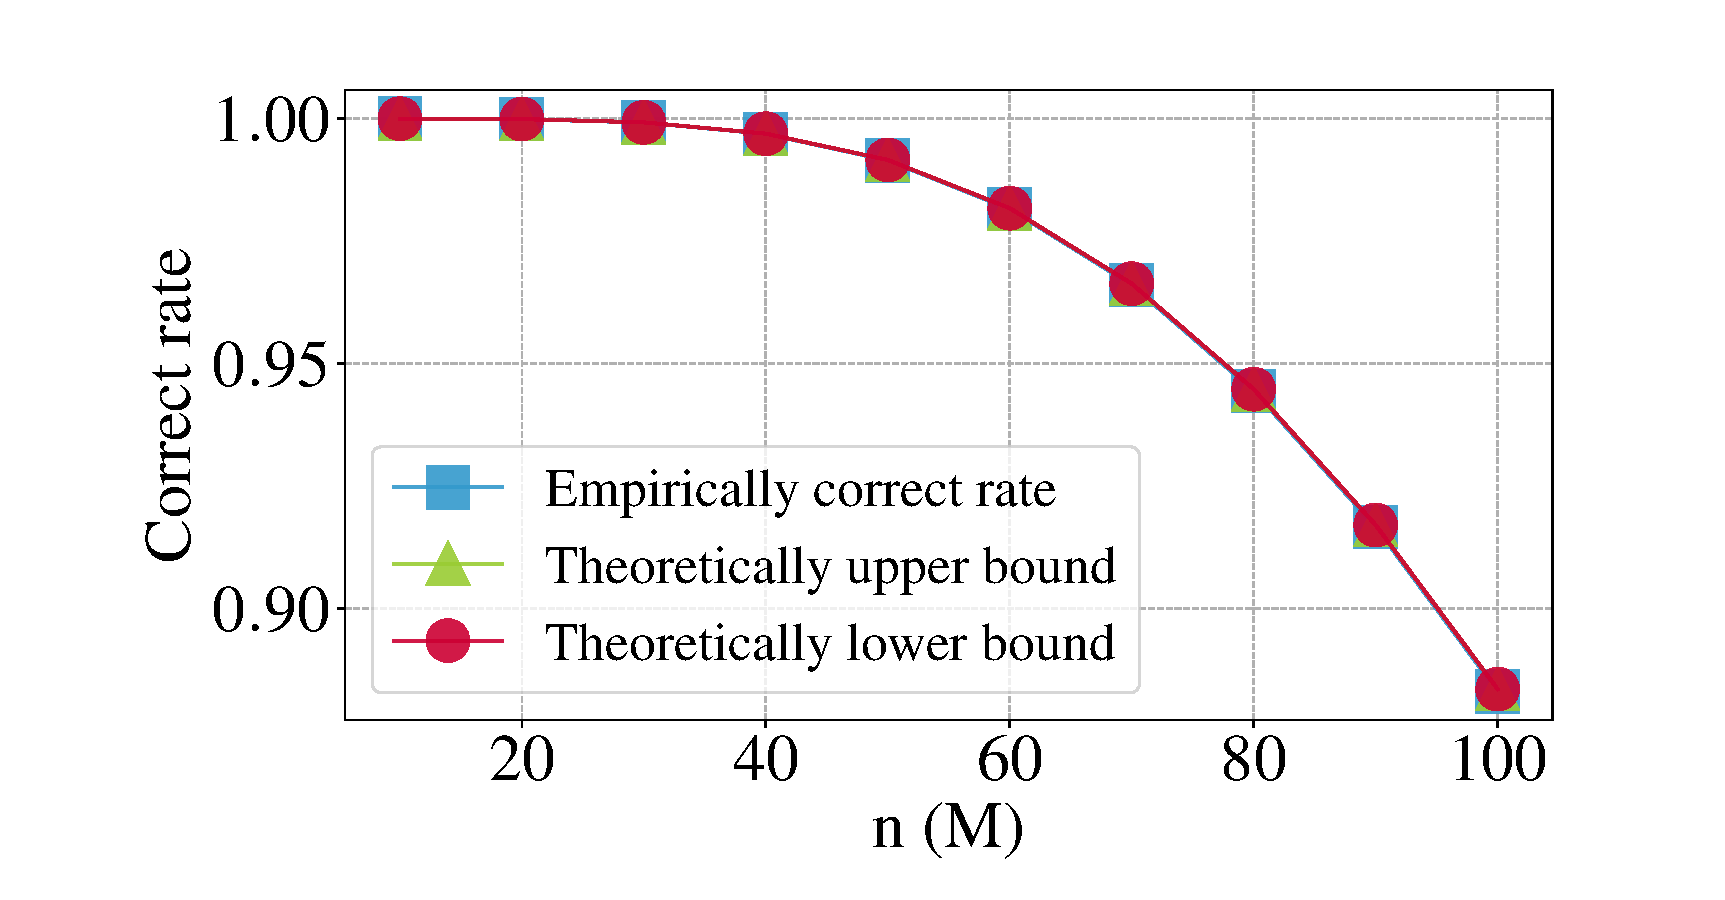
\includegraphics[width=0.90\textwidth, height=1.125in]{cr_n}}
		\postfig\precaption\adjustfigs
%		\vspace{-0.05in}
		\caption{Correct rate vs. $n$ for $m = 500$M and $k = 6$.}
		\label{cr_n}\postcaption
	\end{minipage}
	%
	\begin{minipage}[t]{0.32\textwidth}{
			\prefig
			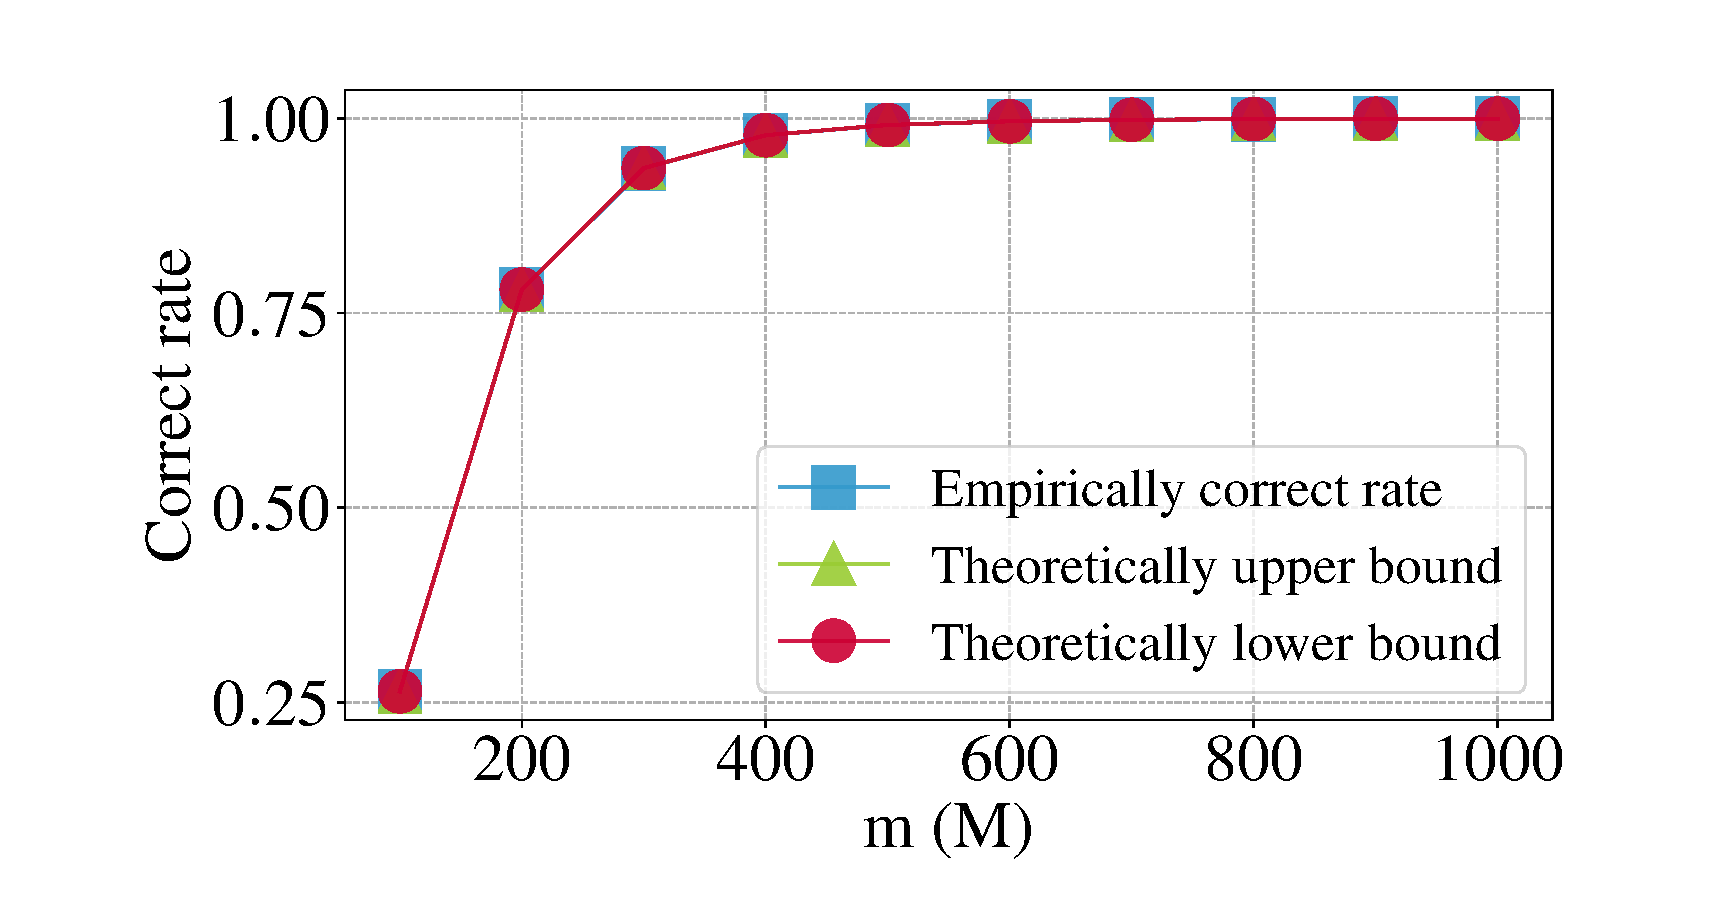
\includegraphics[width=0.90\textwidth, height=1.125in]{cr_m}}
		\postfig\precaption\adjustfigs
%		\vspace{-0.05in}
		\caption{Correct rate vs. $m$ for $n = 50$M and $k = 6$.}
		\label{cr_m}\postcaption
	\end{minipage}
	%
	\begin{minipage}[t]{0.32\textwidth}{
			\prefig
			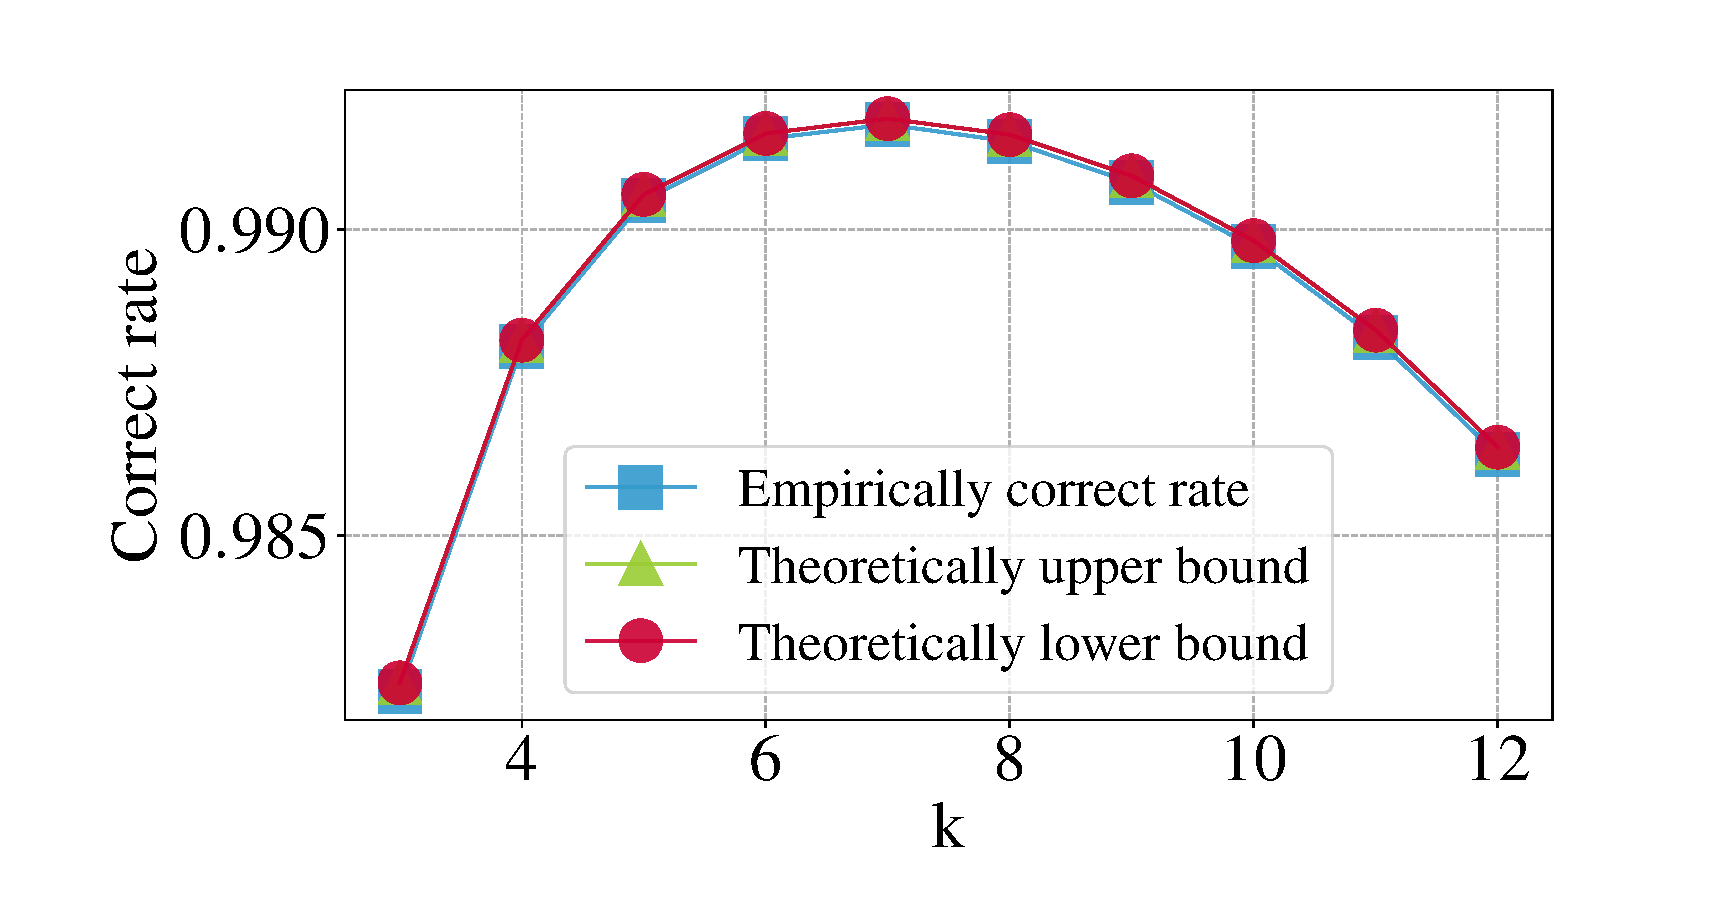
\includegraphics[width=0.90\textwidth, height=1.125in]{cr_k}}
		\postfig\precaption\adjustfigs
%		\vspace{-0.05in}
		\caption{Correct rate vs. $k$ for $n = 50$M and $m = 500$M.}
		\label{cr_k}\postcaption
	\end{minipage}
	%
%	\vspace{-0.03in}
\end{figure*}

\subsubsection{Upper Bound vs. $n$}

Figure \ref{upbound_n} plots the empirical results, Bloom's theoretical results, Bose's upper bounds, and our upper bounds of FP probability with different $n$ increasing from 10M to 100M with a step of 10M for $m = 500$M and $k = 6$. 
\textit{Our results show that our upper bounds of FP probability follows the empirical FP probability very well, regardless of the values of $n$.} 
We find that all above four results almost coincide with each other, which demonstrates the tightness of bounds in Eq. \ref{fBound} and \ref{bounds}. 

To compare upper bound of Bose and ours more intuitively, in Figure \ref{upbound_error_ratio_n}, we plot the bounds error ratios $\beta$, defined as $\beta=\frac{upper\ bound - lower\ bound}{lower\ bound}$, of these two upper bounds with different $n$ increasing from 10M to 100M with a step of 10M for $m = 500$M and $k = 6$. 
\textit{Our results show that the bounds error ratio of our upper bound is $26821.2\sim125492.5$ lower than that of Bose's upper bound. }
We find that our upper bound almost coincides with the lower bound, which demonstrates the superiority of our upper bound. 







%\begin{figure}[htbp]
%	\prefig
%	\centering
%	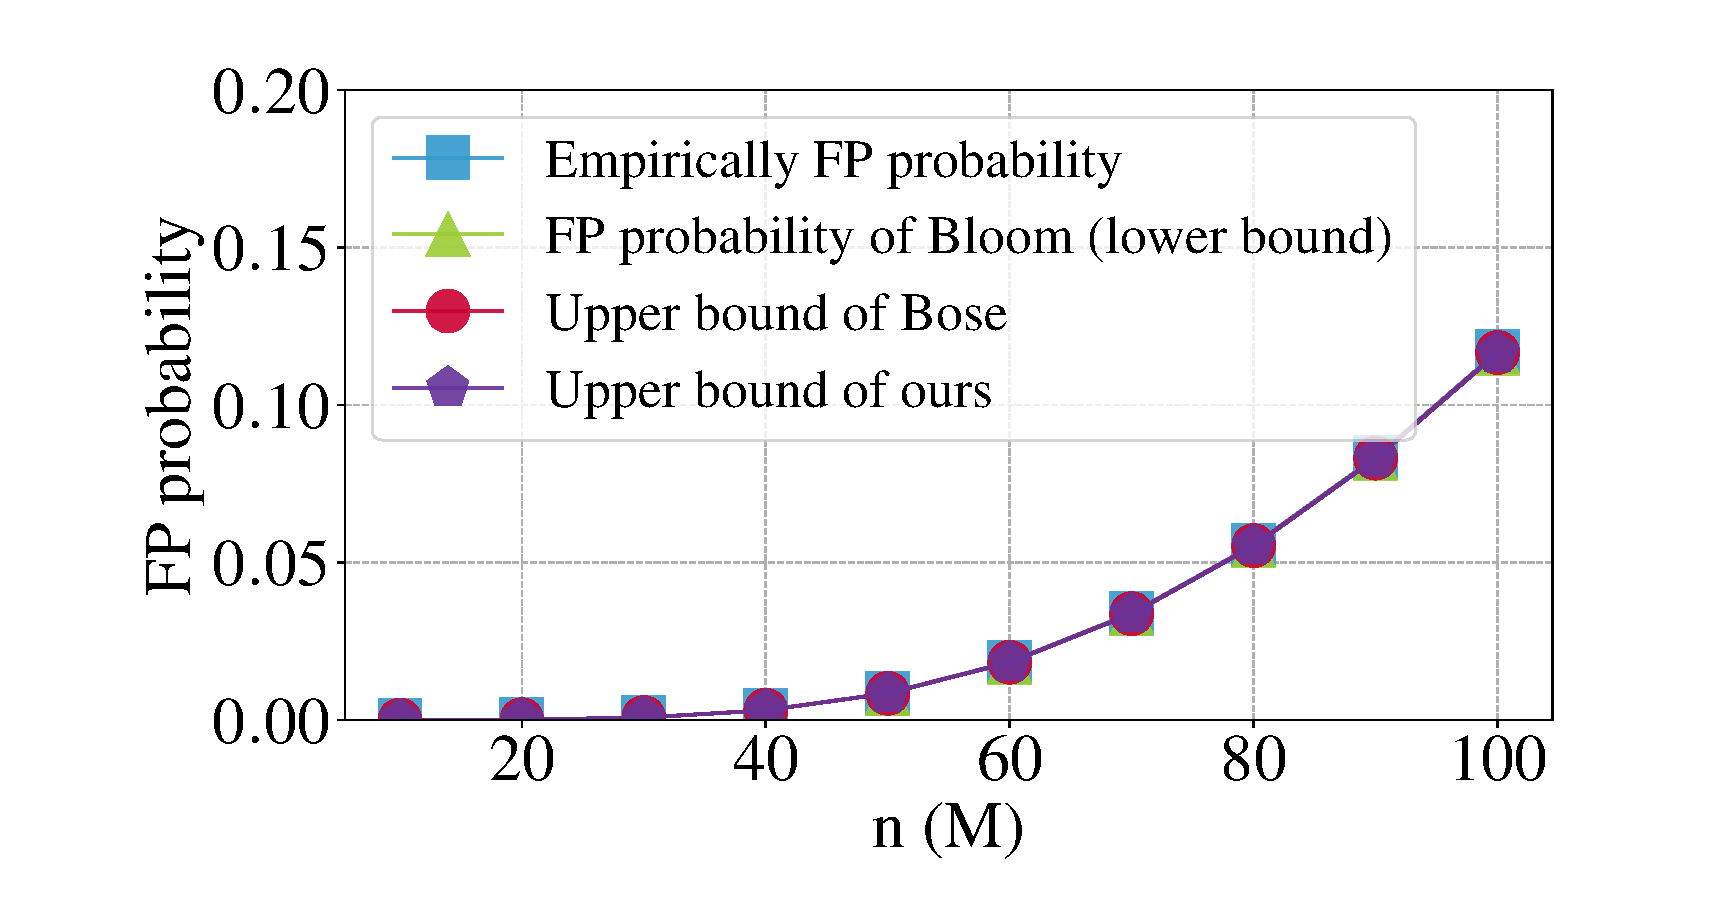
\includegraphics[width=\figwidthdraw]{upbound_n}
%	\postfig\precaption
%	\caption{FP probability vs. $n$ for $m = 500$M and $k = 6$.}
%	\label{upbound_n}
%	\postcaption
%\end{figure}
%
%
%\begin{figure}[htbp]
%	\prefig
%	\centering
%	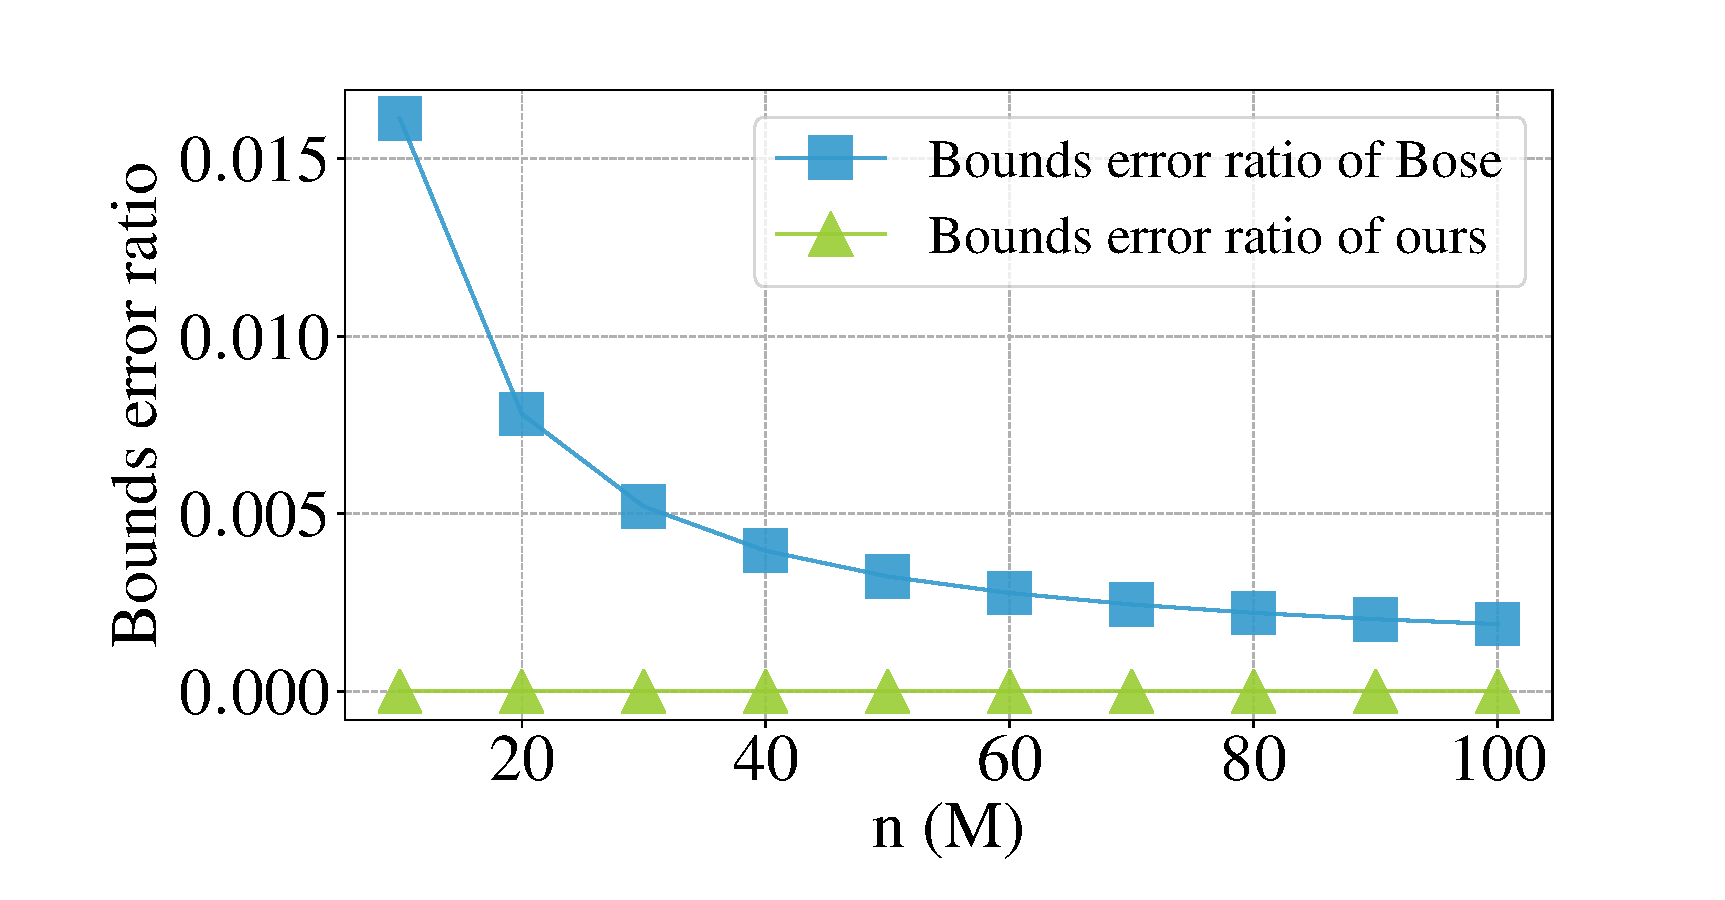
\includegraphics[width=\figwidthdraw]{upbound_error_ratio_n}
%	\postfig\precaption
%	\caption{Bounds error ratio vs. $n$ for $m = 500$M and $k = 6$.}
%	\label{upbound_error_ratio_n}
%	\postcaption
%\end{figure}


\subsubsection{Upper Bound vs. $m$}

Figure \ref{upbound_m} plots the empirical results, Bloom's theoretical results, Bose's upper bounds, and our upper bounds of FP probability with different $m$ increasing from 100M to 1000M with a step of 100M for $n = 50$M and $k = 6$. 
\textit{Our results show that our upper bounds of FP probability follows the empirical FP probability very well, regardless of the values of $m$.} 
%We find that all above four results almost coincide with each other, which demonstrates the tightness of bounds in Eq. \ref{fBound} and \ref{bounds}. 

Figure \ref{upbound_error_ratio_m} plots the bounds error ratios of these two upper bounds with different $m$ increasing from 100M to 1000M with a step of 100M for $n = 50$M and $k = 6$. 
\textit{Our results show that the bounds error ratio of our upper bound is $21885.4\sim150182.6$ lower than that of Bose's upper bound. }
We find that our upper bound almost coincides with the lower bound, regardless of the values of $m$. 


%\begin{figure}[htbp]
%	\prefig
%	\centering
%	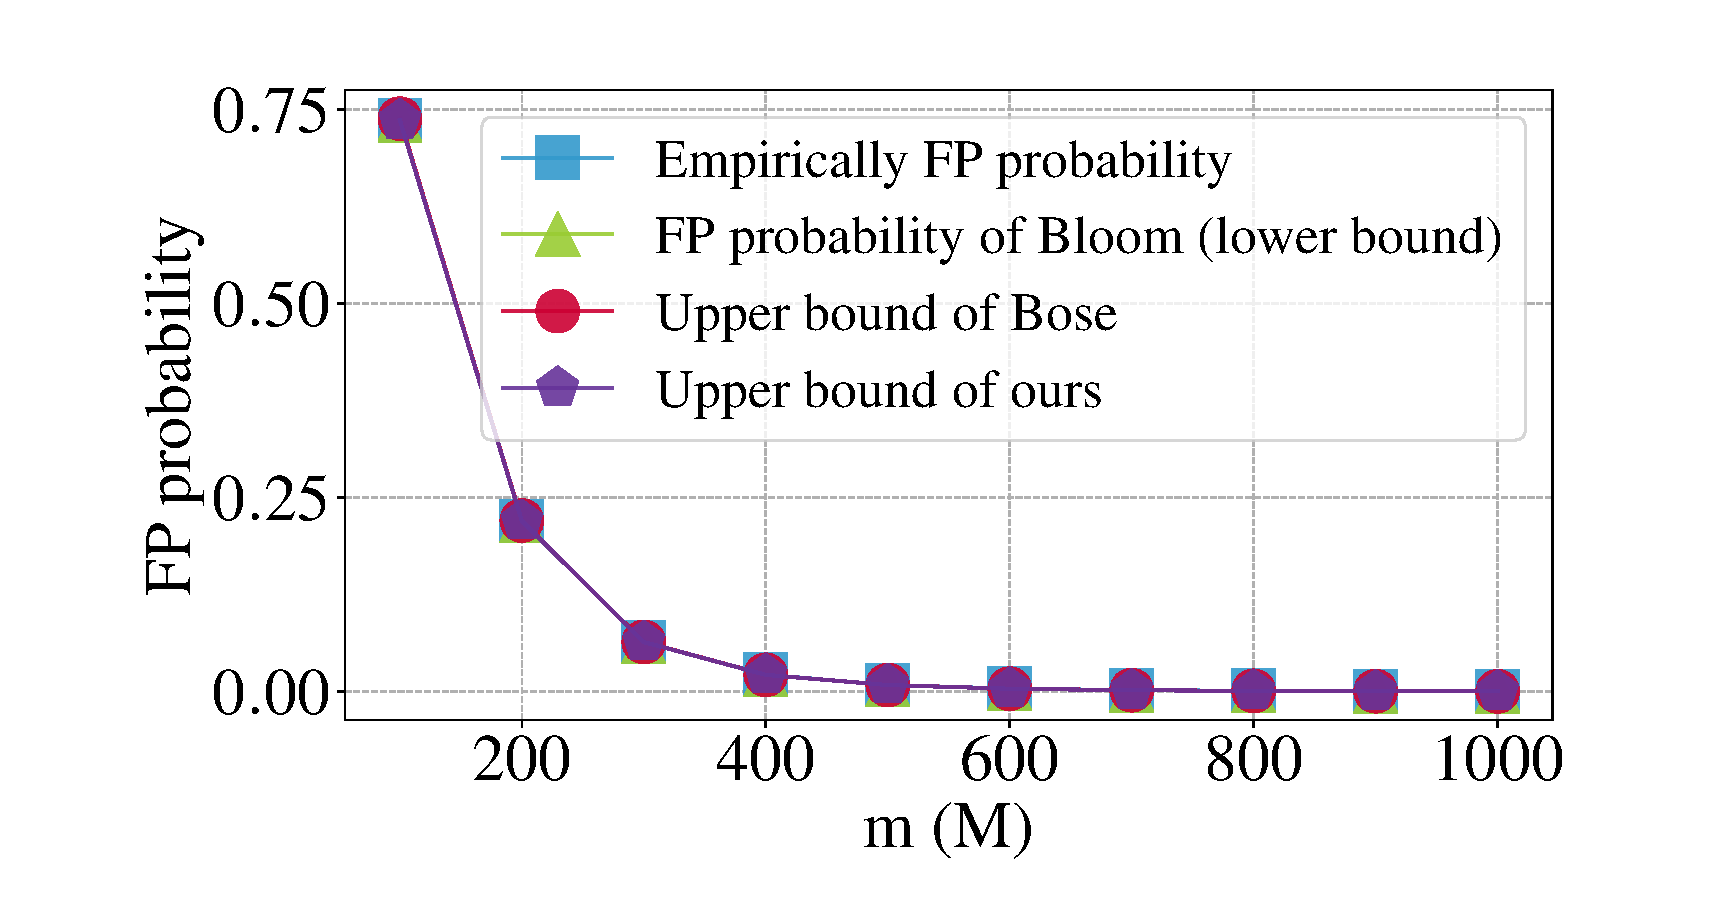
\includegraphics[width=\figwidthdraw]{upbound_m}
%	\postfig\precaption
%	\caption{FP probability vs. $m$ for $n = 50$M and $k = 6$.}
%	\label{upbound_m}
%	\postcaption
%\end{figure}
%
%
%\begin{figure}[htbp]
%	\prefig
%	\centering
%	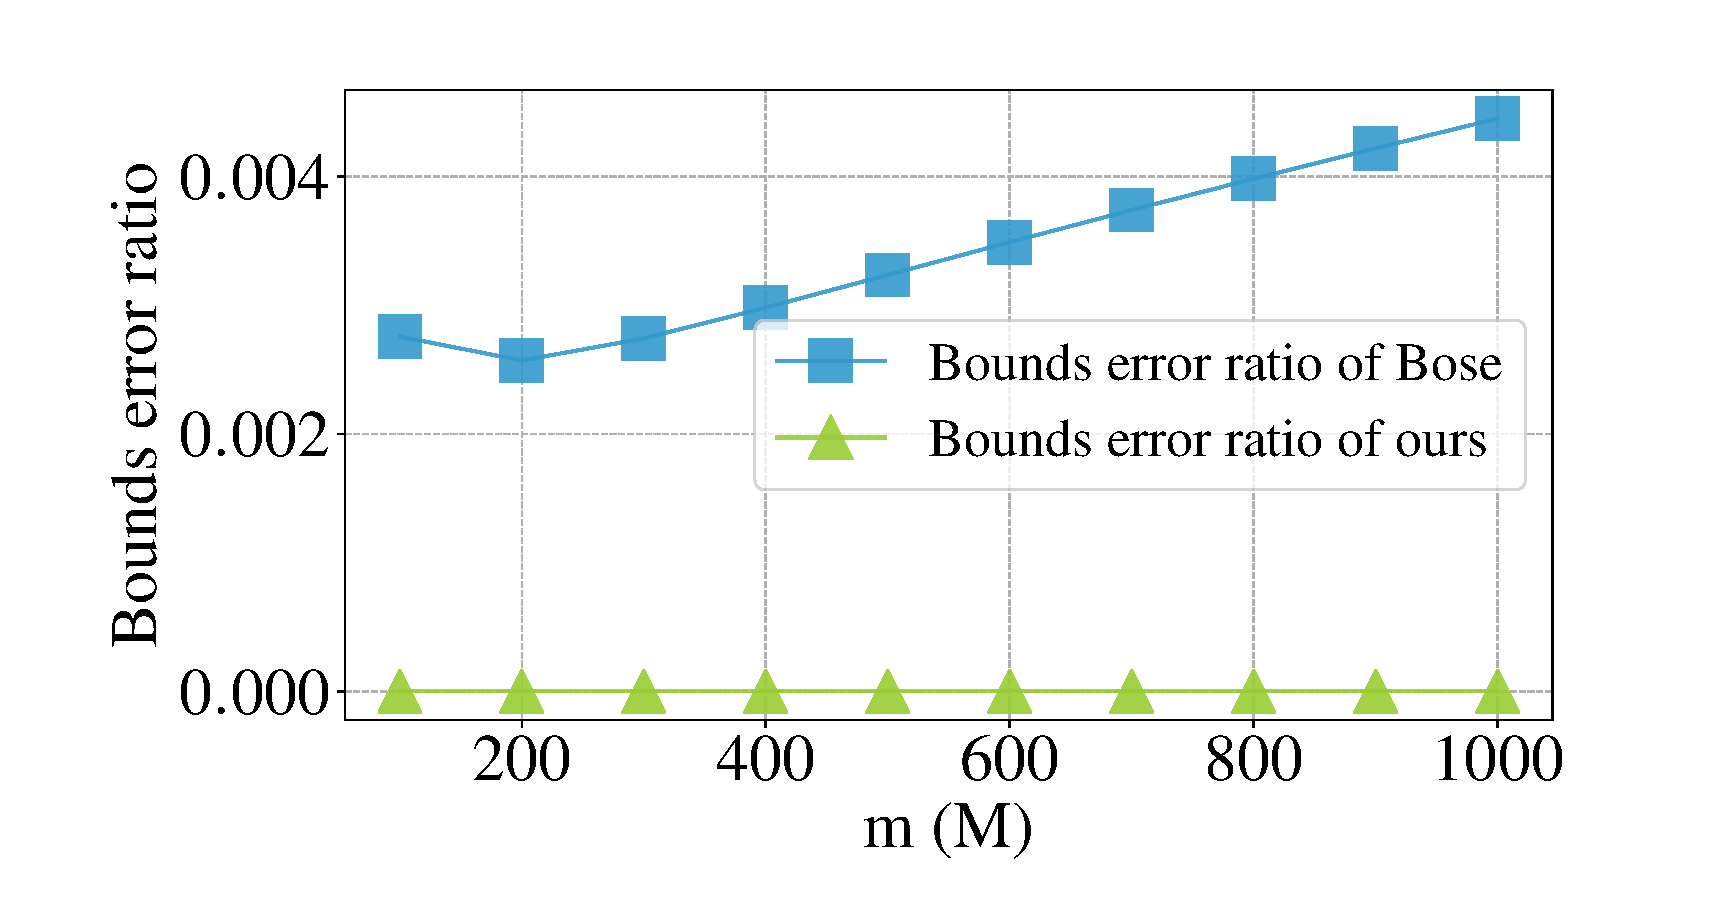
\includegraphics[width=\figwidthdraw]{upbound_error_ratio_m}
%	\postfig\precaption
%	\caption{Bounds error ratio vs. $m$ for $n = 50$M and $k = 6$.}
%	\label{upbound_error_ratio_m}
%	\postcaption
%\end{figure}


\subsubsection{Upper Bound vs. $k$}

Figure \ref{upbound_k} plots the empirical results, Bloom's theoretical results, Bose's upper bounds, and our upper bounds of FP probability with different $k$ increasing from 3 to 12 with a step of 1 for $n = 50$M and $m = 500$M. 
\textit{Our results show that our upper bounds of FP probability follows the empirical FP probability very well, regardless of the values of $k$.} 
%We find that all above four results almost coincide with each other, which demonstrates the tightness of bounds in Eq. \ref{fBound} and \ref{bounds}. 

Figure \ref{upbound_error_ratio_k} plots the bounds error ratios of these two upper bounds with different $k$ increasing from 3 to 12 with a step of 1 for $n = 50$M and $m = 500$M. 
\textit{Our results show that the bounds error ratio of our upper bound is $39483.8\sim64668.5$ lower than that of Bose's upper bound. }
%We find that our upper bound almost coincides with the lower bound, which demonstrates the superiority of our upper bound. 

%\begin{figure}[htbp]
%	\prefig
%	\centering
%	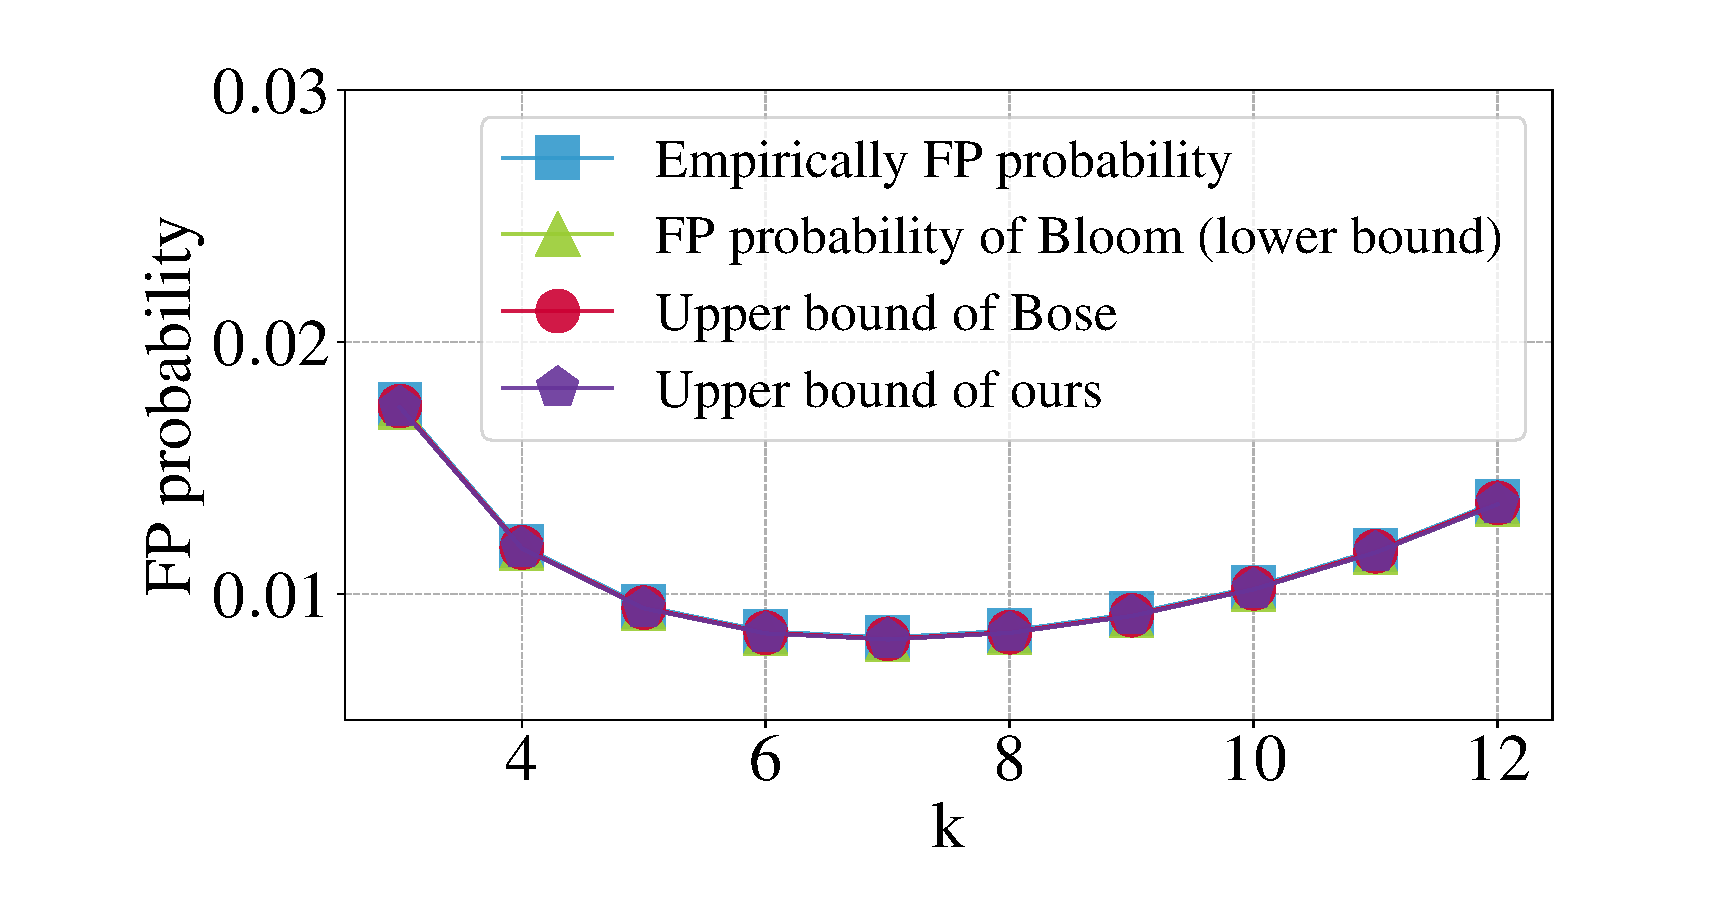
\includegraphics[width=\figwidthdraw]{upbound_k}
%	\postfig\precaption
%	\caption{FP probability vs. $k$ for $n = 50$M and $m = 500$M.}
%	\label{upbound_k}
%	\postcaption
%\end{figure}
%
%
%\begin{figure}[htbp]
%	\prefig
%	\centering
%	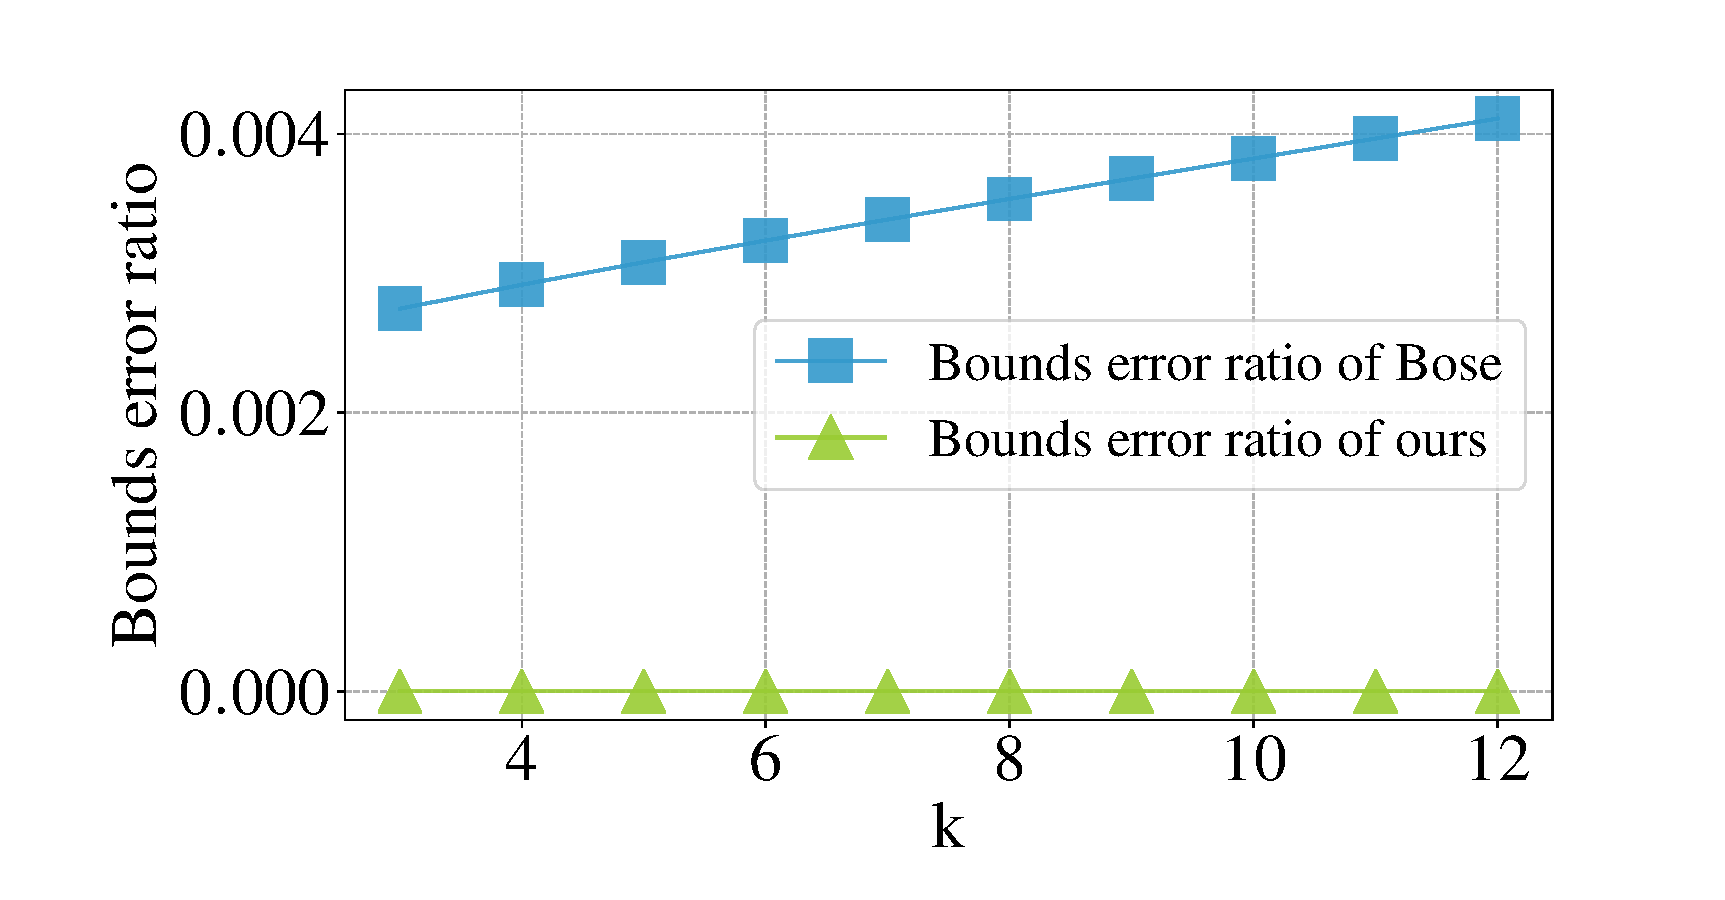
\includegraphics[width=\figwidthdraw]{upbound_error_ratio_k}
%	\postfig\precaption
%	\caption{Bounds error ratio vs. $k$ for $n = 50$M and $m = 500$M.}
%	\label{upbound_error_ratio_k}
%	\postcaption
%\end{figure}

\vspace{-0.05in}
\subsection{$\mathcal{C}_r$ Formula Validation}
\vspace{-0.02in}
Figure \ref{cr_n}, \ref{cr_m}, and \ref{cr_k} plot the correct rates of CFBs with different values of $n$, $m$, and $k$, respectively. 
\textit{Our results show that our lower and upper bounds of the correct rate of CBFs follow the empirical correct rates very well, regardless of the values of $n$, $m$, and $k$.}

 
%
%\subsubsection{Correct Rate vs. $n$}
%
%\subsubsection{Correct Rate vs. $m$}
%
%\subsubsection{Correct Rate vs. $k$}

%\section{Related Work}
\label{sec:relatedwork}

%Given a set of $n$ elements, given a array of $m$ bits, 
Given a set of $n$ elements as well as a array of $m$ bits, using $k$ hash functions to read $k$ bits of the array, Bloom Filter can judge whether an element belongs to this set. That an element not belonging to the set is judged to be is called false positive. Bloom Filter shows  how to achieve the minimal false positive probability in theory. 

The membership query speed is fast, thus BFs are applied to various fields.  Specifically, after 2003, Bloom Filters are widely applied in computer network filed \cite{sig03PBF, songsig05, BFDanLi, yuConext09, BF_TC}. A comprehensive survey of Bloom Filter is provided in \cite{BFSurvey9C}.

The main shortcoming of Bloom Filters is the false positive, which can hardly be improved because it is proven to be optimal in theory. Therefore, although various papers proposed to improve the standard Bloom Filter (SBF), few of them are really effective. Here we only survey the significant improvement of Bloom Filters below. 

The improvement of Standard Bloom Filter (SBF) can be divided into four kinds: counter-oriented filters, false positive-oriented filters, overhead-oriented filters, and other filters.

\subsection{Counter-oriented Filters}
Because there is only one bit for each hash position, thus SBF cannot support deletion, while it supports insertion naturally. 
To address this issue, Counting Bloom Filter (CBF) which uses a counter (usually 4 bits) to replace a bit in one hash position is proposed in \cite{webcaching}. The cost of supporting deletion is several times of space requirement and false negative. When a counter in a CBF ever overflows, the standard CBF just let it stay at its maximum value. After many deletions, the counter may decrease to 0 while it shouldn't be, then false negative might happen. Fortunately, the probability of false negative is very small \cite{falsenegative}.
%When a counter in a CBF overflows, after many deletion, when this counter decreases to 0, false negative might happen. Fortunately, the probability of false negative is very small \cite{falsenegative}.%

Based on CBF, Spectral BF \cite{spectralBF} can not only supports membership query, but also tells that the probability that one element appears in the set.

\subsection{False Positive-oriented Filters}
To make a trade-off between false positive and false negative, retouched Bloom filters are proposed in \cite{retouchedBF}. Its application range is confined in those which allow both small false positive and false negative. 

The false positive of Bloom Filter is optimal in theory, thus it cannot be compressed. Actually, it is optimal for the three parameters: size ($m$), the number of hash functions ($k$), the number of elements ($n$). When other parameters are introduced, the optimal formula changes. 
Based on this observation, besides $n$, $k$, $m$ (the size before compression), when the size after compression $z$ is introduced, the optimal false positive changes. Compressed Bloom filter is proposed in the situation where Bloom filter is passed as a message \cite{compressedBF}. 

\subsection{Overhead-oriented Filters}
Since it is hard to optimize the false positive, some work focus on the improvement of the overhead of BF queries. 
In many applications, Bloom Filter is small enough to be stored in on-chip memory (such as CPU and GPU cache). When BFs are stored in on-chip memory, the overhead hash computation cannot be ignored compared with memory access, because one memory access of on-chip memory only needs several clock cycles. To reduce the overhead of hashing, Kirsch \etal propose to use two hash functions to simulate $k$ hash functions at the cost of the increase of false positive probability \cite{lessHashBF}.


Qiao \etal propose to confine the $k$ hash positions in one or several words \cite{onemem}. In this way, the number of memory accesses can be significantly reduced. Similar with Kirsch's solution, the cost is the increase of false positive probability. Both of these two papers claimed that the increased false positive probability is small.

\subsection{Other Filters}

Besides membership query, some add additional functions to SBF, such as Bloomier filter \cite{Bloomier}, and Dynamic bloom filters \cite{DynamicBF}. 
Some focus on the choice of hash functions, such as Bloom Filters using universal hashing \cite{universalHash}, and Bloom Filters with practical hashing \cite{partitionHashBF}.
Some focus on the problem of multiple sets and BFs, such as 
d-Left filters \cite{dleft}, DLB-BF \cite{songV6}, Multi-class
Bloom Filter \cite{BFDanLi},  Bloom Filter for set query \cite{setqueryBF}, Combinatorial Bloom Filters \cite{combineBF}, and BloomCast \cite{BloomCast}.




%Bloom Filter is applied into many fields, and its applications can be divided into the following four categories:

%1) cache judgment.
%2) IP lookups.
%3) MAC address lookup.
%4) packet classification.
%
%There is also another classification method:
%1) single Bloom Filter application.
%2) multiple Bloom Filters application.

%talk about the BFs in which classification method????



%Although so many variants of Bloom Filters are proposed, the standard BF continues to be the most popular in a great number of applications owing to its simplicity and outstanding performance. 
\section{Conclusion}
\label{sec:conclusion}
%\vspace{-0.2in}
In this paper, we discuss the controversy of the formula of Bloom Filter. Three formulas of false positive probability are presented: Bloom's formula, Bose's formula, and Christensen's formula. There is an error in the deduction process of Bloom's formula, and a minor error in Bose's formula. Christensen's formula is correct, but the false positive must be caculated using an iterative table-based algorithm with a time complexity of $O(knm)$. What is worse, it cannot deduce the optimal value of $k$.
%Christensen's formula is correct, but can only compute the false positive when $m$ is small, it cannot deduce the optimal value of $k$.


To compute the optimal value of $k$, we use information and entropy theory to deduce the exact formula of $k$.
To compute the false positive probability, 1) For small $m$, Christensen's formula can be used; 2) For large $m$, we propose a new upper bound which is much more accurate than state-of-the-art. Fortunately, when $m$ is infinitely large, our upper bound becomes the same as the lower bound, which is Bloom's formula.
Besides, we derive the bounds of correct rate of counting Bloom filters through our proposed formulas about Bloom filters. 
All the implementation source code is made publicly available anonymously at GitHub \cite{opensource}.
%we prove a limit form of false positive probability using left and right limit, and find out that it is same as Bloom's. 
%3) We also show that the error is negligible when $m$ is not large using two simple examples.
\newpage \balance
 
\bibliographystyle{IEEEtran}
\bibliography{reference}
\end{document} 